\documentclass[12pt]{book}
%paquetes
\usepackage[spanish,es-tabla]{babel}
\usepackage[utf8]{inputenc}
\usepackage[pdftex,colorlinks=true,bookmarks=true,linkcolor=black,urlcolor=black,citecolor=black,pdfencoding=unicode]{hyperref}
\usepackage{bookmark}
\usepackage{appendix}
\usepackage{subfig}
\usepackage[dvips]{graphicx}
\usepackage{multicol}
\usepackage{multirow}
\usepackage{array,color}
\usepackage{booktabs}
\usepackage[neverdecrease]{paralist}
\usepackage{array}
\usepackage{listings}
\usepackage[nottoc]{tocbibind}
\usepackage{datetime}
\usepackage{algorithmicx}
\usepackage{algpseudocode}
\usepackage[ruled]{algorithm}
\usepackage[letterpaper]{geometry}
\usepackage{emptypage}
\usepackage{pdfpages}
%\usepackage[showframe,letterpaper]{geometry}
%\usepackage{lmodern}
%\usepackage{layouts}
%\usepackage{boxedminipage}
% \usepackage{fancyhdr}% manipulación de encabezados y pie de pagina
% \usepackage{anysize}% Permite emplear cualquier medida de márgenes. 
% \usepackage{titlesec}%estilo de secciones, títulos ....
% \usepackage[usenames]{color}
% \usepackage{graphicx}
% \usepackage{color}
%\usepackage{setspace}
%\usepackage{enumitem}
%\usepackage{emptypage}
%\usepackage{soul}
%\usepackage{ragged2e}

%% Definiciones %%
\floatname{algorithm}{Algoritmo}
\renewcommand\tocbibname{Referencias}
% \definecolor{Black}{rgb}{0,0,0}
\title{Idónea Comunicación de Resultados}
\author{Angel González Méndez}
%\date{2014-09-01}

%% Comandos %%
\newdateformat{mydate}{\monthname[\THEMONTH] de \THEYEAR}
\newcommand{\zespacio}{\linebreak \linebreak}
\newcommand{\despacio}{\linebreak \linebreak \linebreak}
\newcommand{\vespacio}{\linebreak \linebreak \linebreak \linebreak}
\newcommand{\fespacio}{\linebreak \linebreak \linebreak \linebreak \linebreak}
\newcommand\barra{\hrule height 2pt}
%\providecommand*{\monthnamespanish}[1]{%
\renewcommand{\monthnamespanish}[1][\month]{%
\ifcase#1\relax
\or Enero%
\or Febrero%
\or Marzo%
\or Abril%
\or Mayo%
\or Junio%
\or Julio%
\or Agosto%
\or Septiembre%
\or Octubre%
\or Noviembre%
\or Diciembre%
\fi}


%% Estilo de pagina %%
\geometry{letterpaper,
tmargin=25mm,
bmargin=25mm,
lmargin=30mm,
rmargin=30mm,
%marginparsep=0mm
}
%\voffset=-36pt
%\marginparsep=20pt
%\textwidth 6.0in
%\textheight 8.75in
%\oddsidemargin 0.4in
%\evensidemargin 0in
% \fancyhf{}
% \pagestyle{fancy}
% \fancyfoot[R]{\thepage}%alineación del pie
% %\fancyhead[OE]{\fancyhead}%alineación del encabezado
% %otros
%\selectspanish
% \marginsize{2.0cm}{2.0cm}{2.0cm}{2.0cm}% Controla los márgenes {izquierda}{derecha}{arriba}{abajo}.
%\colorbox{color}{texto} % remarcar texto con color

%% Estilo Parrafo y listas %%
%\spacing{1.5}
%\setlength{\parindent}{0pt}
%\renewcommand{\baselinestretch}{1.5}
%\linespread{1.5}

\newcommand{\hiddensubsection}[1]{
    \stepcounter{subsection}
    \subsection*{\arabic{chapter}.\arabic{section}.\arabic{subsection}\hspace{1em}{#1}}
}

\begin{document}
%	\pagebreak
%	\printinunitsof{mm}{\pagevalues}
%	\verb|\marginparwidth|: \printinunitsof{mm}\prntlen{\marginparwidth}
%	\pagediagram
%	\pagebreak
 	\frontmatter
 	\addtocontents{toc}{\barra}
 	\cleardoublepage
 	% \begin{center}
% 	\thispagestyle{empty}%quitar encabezado, pie y numero de pagina
% 	\begin{huge}
% 		\textbf{Universidad Autónoma Metropolitana} \despacio
% 	\end{huge}
% 	\begin{large} 
% 		Unidad Azcapotzalco \linebreak
% 		División de Ciencias Básicas e Ingeniería \linebreak
% 		Ingeniería en Computación \zespacio
% 		Proyecto Terminal de Ingeniería en Computación\zespacio
% 	\end{large}
% 
% 	\begin{LARGE}
% 	\begin{center}
% 		\textbf{ Codificación Concurrente de Audio en Arquitecturas Multi-Núcleo}\zespacio
% 	\end{center}
% 	\end{LARGE}
% 
% 	\begin{large}
% 		\textbf{Reporte Final}\despacio
% 		Alumno: \linebreak
% 		\textbf{González Méndez Angel - 206308547} \zespacio
% 		Fecha de entrega: \linebreak
% 		\textbf{06 / septiembre / 2010} \zespacio
% 		Trimestre Lectivo: \linebreak
% 		\textbf{10-P} \zespacio
% 		Asesor: \linebreak
% 		\textbf{M. en C. Oscar Alvarado Nava - 26424}
% 	\end{large}
% \end{center}

\thispagestyle{empty}
\oddsidemargin 0.0in
\begin{minipage}[t]{\textwidth}
	\begin{center}
	 	\includegraphics[width=\textwidth]{img/variacion3Izt.png}
	\end{center}
\end{minipage}

\oddsidemargin 0.2in
% \begin{minipage}{0.82\textwidth}
% \begin{center}
% 	\normalsize \sc Universidad Autónoma Metropolitana \\
% 	Unidad Azcapotzalco
% \end{center}
% \end{minipage}

%\vspace{1.5cm}
%\centerline{\Large{\bf Universidad Autónoma Metropolitana}}
%\vspace{0.5cm}
%\centerline{\Large \bf Unidad }

\vspace{1.5cm}
%\centerline{\Large \bf Departamento }
\centerline{\large  División de Ciencias Básicas e Ingeniería}
\vspace{0.5cm}
\centerline{\large Posgrado en Ciencias y Tecnologías de la Información}
\vspace{0.5cm}
\centerline{\large  Idónea Comunicación de Resultados}

\vspace*{\stretch{1}}
\begin{center}
\Large \bf
Propuesta de un Sistema Paralelo para la Creación de Redes Porosas sujetas a Restricciones Geométricas en Arquitecturas Multicore
\end{center}
\vspace*{\stretch{1}}

%\centerline{\Large \bf Tesis que presenta:}
\centerline{\normalsize presenta:}
%\vspace{0.5cm}
\vspace{0.1cm}
\centerline{\Large \bf Ing. Angel González Méndez}
\vspace{0.5cm}
%\centerline{\Large \bf para obtener el Grado de}
\centerline{\normalsize para obtener el Grado de:}
%\vspace{0.5cm}
\vspace{0.1cm}
\centerline{\Large \bf Maestro en Ciencias}
\centerline{\Large \bf (Ciencias y Tecnologías de la Información)}
\vspace{1.0cm}
\centerline{Asesor del Proyecto:}
\vspace{0.1cm}
\centerline{\Large \bf Dra. Graciela Román Alonso}
\vspace{0.5cm}
%\centerline{\Large \bf [Nombre del Director(a)/Codirectores(as)]}
 
\vspace{1.2cm}
{\large \bf México, D.F. \hfill  \mydate\today}

\cleardoublepage
 	%\setlength{\parindent}{default}
 	\cleardoublepage
	%\chapter{Resumen}
%\bigskip
%\barra
%\bigskip
%\thispagestyle{empty}
%El estudio de materiales porosos es de gran importancia para un gran número de aplicaciones industriales, con el fin de estudiar características especificas de los materiales o procesos fisicoquímicos de los mismos(ej. simulación in-silico). Este trabajo tiene como base el Modelo Dual de Sitios y Enlaces(DBMS). Bajo este enfoque se tiene que un material poroso se compone por sitios(cavidades, protuberancias) los cuales están interconectados a través de enlaces; cada sitio se interconecta con una serie de enlaces y cada enlace interconecta a dos sitios. En la actualidad, varios algoritmos computacionales se han implementado, sin embargo, solo unos cuantos validan las restricciones geométricas que surgen al conectar un sitio con sus respectivos enlaces en una red porosa. Al validar este tipo de restricciones nos ayudaría a la creación de redes porosas más cercanas a la realidad. En este trabajo, se proponen dos soluciones para la construcción de redes porosas sujetas a restricciones geométricas es decir se validan las restricciones geométricas entre todos los poros de una red porosa, cada algoritmo se implemento de forma secuencial y paralela. Nuestras propuestas paralelas fueron implementadas utilizando OpenMP para que a través de crear un conjunto de hilos (tareas computacionales), estos trabajen de forma simultanea en regiones aleatorias e independientes de una red porosa y de esta forma disminuir sustancialmente los tiempos de creación.


%% OK
\chapter{Resumen}
\bigskip
\barra
\bigskip
\thispagestyle{empty}
El estudio de los medios porosos se realiza con el fin de entender las caracter\'isticas espec\'ificas de los materiales o procesos capilares de los mismos, es de gran importancia para un gran n\'umero de aplicaciones industriales. El Modelo Dual de Sitios y Enlaces (DBMS, por sus siglas en ingl\'es) ha sido una base importante en el desarrollo de simuladores (in-silico) de medios porosos. Bajo este enfoque, se tiene que un material poroso se compone por sitios(cavidades, protuberancias) los cuales est\'an interconectados a trav\'es de enlaces; cada sitio se interconecta con una serie de enlaces y cada enlace interconecta a dos sitios. En la actualidad, varios algoritmos computacionales para la simulaci\'on de redes porosas se han implementado, sin embargo, solo unos cuantos validan el cumplimiento de las restricciones geom\'etricas que surgen al conectar dos enlaces adyacentes de un mismo sitio, en donde no debe existir interferencia espacial entre ellos. El validar este tipo de restricciones nos ayuda a crear redes porosas m\'as realistas; sin embargo, la complejidad algor\'itimica que conlleva el cumplimiento de estas restricciones hace que el tiempo de construcci\'on de una red aumente. En este trabajo, se parte de un algoritmo secuencial desarrollado como parte del Proyecto Interdisciplinario de los Departamentos de Ing. El\'ectrica y de Qu\'imica de la UAM-IZT, el cual genera redes porosas que incluyen las restricciones geom\'etricas; el inconveniente de este algoritmo es que requiere de largo tiempo para construir redes porosas grandes. Para solucionar dicho aspecto, se proponen dos versiones paralelas de construcci\'on de redes porosas, validando las restricciones geom\'etricas entre todos los poros, bas\'andonos en el DBSM. El objetivo de la primer propuesta es paralelizar el algoritmo secuencial anteriormente desarrollado, mientras que la seguna propuesta aplica el M\'etodo de Monte Carlo paralelo en la construcci\'on de una red porosa.  Nuestras propuestas paralelas fueron implementadas bajo un modelo de memoria compartida, usando OpenMP para crear un conjunto de hilos (tareas computacionales) los cuales trabajan de forma simult\'anea en espacios aleatorios e independientes.

	\cleardoublepage
	\cleardoublepage
\nopagebreak
\chapter{Agradecimientos}
\bigskip
\barra
\bigskip
%\thispagestyle{empty}

\noindent{
A mi madre Lucía Guadalupe Méndez González, por creer en mi en todo momento, por su apoyo incondicional a lo largo de mi vida y por ser un ejemplo de vida.\\
}

\noindent{
A mi padre Hilario González Estrella, a pesar de que ya no te encuentras con nosotros, tu espíritu siempre a estado conmigo.\\
}

\noindent{
A mi hermanas, de las cuales siempre he recibido su apoyo.\\
}

\noindent{
A mi tutora la Dra. Graciela Román Alonso, por su constante apoyo para la realización de este trabajo.\\
}

\noindent{
A los profesores del Posgrado en Ciencias y Tecnologías de la Información, por todos los conocimientos otorgados en sus clases, los cuales fueron la base para hacer posible el presente trabajo.\\
}

\noindent{
A la Universidad Autónoma Metropolitana - Iztapalapa, por las facilidades otorgadas para el correcto desarrollo del este trabajo y por permitirme formar parte de esta gran institución.\\
}

\noindent{
Al Laboratorio Supercómputo y Visualización en Paralelo, por los recursos prestados, sin los cuales esto trabajo no hubiera sido posible.\\
}

\noindent{
Al Consejo Nacional de Ciencia y Tecnología, por el apoyo económico otorgado a través de su programa de becas para la realización de mis estudios de posgrado.
}



	\cleardoublepage
	\addtocontents{lot}{\barra}
 	\addtocontents{lof}{\barra}
 	%\addtocontents{loa}{\barra}
 	\addcontentsline{toc}{chapter}{Índice general}
	\tableofcontents
	\cleardoublepage
	\listoffigures
	\cleardoublepage
	%\listofalgorithms
	%%\addtocontents{loa}{\def\string\figurename{Algorithm}}
%	\cleardoublepage
%	\listoftables % indice de tablas
%	\addcontentsline{toc}{chapter}{Lista de figuras} % para que aparezca en el indice de contenidos
%	\addcontentsline{toc}{chapter}{Lista de tablas} % para que aparezca en el indice de contenidos
	\mainmatter
	\chapter{Introducción}
\label{champ:intro}
\bigskip
\barra
\bigskip

\section{Computo Paralelo y Simulación por Computadora}
\label{sec:cp}

Por años se han utilizado las computadoras como herramientas para la solución, aproximación o simulación de problemas científicos reales, los cuales tienen una o varias de las siguientes características: son complejos, requieren de un gran número de cálculos o manipulan grandes volúmenes de datos. Lo anterior fue la razón por la cual nació la computación científica la cual es una actividad multidisciplinaria en la cual se hacen uso de métodos y técnicas computacionales para dar soluciones exactas o aproximadas con la premisa de que al utilizar las computadoras el tiempo para obtener resultados es menor. Por lo general la computación científica hace uso  del computo de alto rendimiento(computo paralelo) a través de modelos de programación paralela, los cuales permiten disminuir el tiempo para obtener resultados así como el uso eficiente de los recursos computacionales.\\

La simulación por computadora es una herramienta altamente utilizada debido a que nos permite obtener soluciones aproximadas sobre escenarios de la vida real, varios ramas de la ciencia hacen uso de simulaciones por computadora para lograr mejores resultados en experimentos reales basándose en la información obtenida de simulaciones. Cuando se habla de simulación por computadora esta inherente que se requiere de un modelo el cual nos ayude a abstraer características y limitaciones de un problema real. Adicionalmente de que la simulación por computadora nos permite generar experimentos con mayor exactitud esta también nos puede ayudar a disminuir riesgos y ahorrar recursos.\\

El computo paralelo fue posible gracias a los avances tecnológicos como lo fueron las computadoras multi-procesador o los primeros clusters(Beowulf), en ambas arquitecturas hubo un avance significativo en la primera fue la incorporación de más de un procesador en una misma tarjeta y en la segunda fue el uso de la capacidad de cómputo de computadoras independientes a través de su interconexión(cluster). En la actualidad el computo paralelo va cobrando mayor fuerza y ademas conforme pasa tiempo se esta volviendo más accesible y por lo mismo se esta aplicando en un mayor número de áreas de conocimiento. En particular para aplicar el computo paralelo en un problema se requiere elegir una arquitectura y un técnica de programación. Las arquitecturas más utilizadas para el cómputo paralelo o de alto rendimiento son: multi-procesador, multi-núcleo, gpus, clusters y grids. Por su parte sobre técnicas de programación lo podemos dividir en 3 grandes grupos: la programación con memoria compartida o la programación con memoria distribuida o programación híbrida. 



Algunos ejemplos donde se ha aplicado el cómputo paralelo para dar una solución en un menor tiempo son: problemas matemáticos , problemas de optimización, así como la simulación de problemas de diversas aréas de conocimiento por mencionar algunos. 


En cuanto a la simulación por computadora

%\cite{mchybrid}
%\cite{mcmulticore}
%\cite{mcdynamically}
%
%\cite{sibalancing}
%\cite{sicloud}
%\cite{sikdtree}
%\cite{silscale}
%\cite{sinfusion}
%\cite{siovercomming}
%\cite{siprocess}

Tanto en \cite{mchybrid} y \cite{mcmulticore} hacen uso de las arquitecturas multi-núcleo sobre memoria compartida para la solución de un problema algebraico y de optimización respectivamente.


Una de las ventajas más notables de la programación mediante memoria compartida en arquitecturas multi-núcleo(CPU) es que la comunicación entre los CPUs y la memoria no supone un cuello de botella es por esto que sigue siendo una de las alternativas para paralelizar un algoritmos. Por ejemplo en 


En este trabajo se hace uso de una arquitectura multi-núcleo y la técnica de programación utilizada es con memoria compartida.\\


Cuando se utilizan arquitecturas multi-núcleo la programación paralela se realiza a través de hilos(tareas computacionales), dos de las tecnologías más utilizadas para el manejo de hilos son: Posix Threads\cite{ref13} y OpenMP\cite{ref6}, ambos siguen el modelo fork-join, sin embargo OpenMP proporciona una interfaz de alto nivel que permite al programador concentrar la mayor parte del tiempo en resolver el problema aplicando algún modelo de programación paralela y no en aspectos técnicos que en ocasiones generan errores que no se relacionan con el problema que se quiere resolver. Ademas OpenMP es un estándar avalado por diversas empresas internacionales y se encuentra soportado por los principales compiladores de C/C++ y Fortran.\\

En particular este proyecto hace énfasis en la simulación de materiales porosos, donde tal y como su nombre lo dice son materiales que tienen poros o huecos, estos poros son de distintos tamaños y se encuentran distribuidos en todo el material con la peculiaridad de que dichos poros se encuentran conectados entre si. Debido a las características que tienen los materiales porosos son altamente utilizados en la industria, al estudiar la estructura y propiedades de estos materiales y adicionalmente con la simulación por computadora se pueden encontrar nuevas aplicaciones y usos industriales.\\

\section{Construcción de Redes Porosas}
\label{sec:costruction}

\subsection{Modelado de Redes Porosas}
\label{subsec:model}
Existen diversos modelos para la simulación de materiales porosos algunos se enfocan en los procesos o fenómenos que suceden dentro de los mismos y otros en la representación del material por si mismo, este último tiene la ventaja de que además de poder conocer las características especificas del material también podemos simular procesos y fenómenos dentro del mismo. Uno de los modelos teóricos para obtener un adecuada descripción de la estructura y propiedades de un medio poroso es el Modelo Dual de Sitios y Enlaces(MDSE)\cite{ref2}, en este modelo existen dos tipos de huecos o poros: sitios y enlaces, donde cada sitio está conectado con un determinado número de enlaces llamado conectividad de la red($C$).\\

La representación Modelo Dual de sitios y Enlaces(MDSE) se puede observar en la Figura \ref{fig:dbsm} en la cual se observa la representación de un medio poroso. Existen varias aplicaciones relacionadas con el MDSE algunas de ellas se reportan en \cite{ref8} y \cite{ref10}. En particular los algoritmos presentados en \cite{ref2}, \cite{ref3} y \cite{ref4} para la creación de redes porosas y en \cite{ref7} para la simulación de la porosimetría del mercurio se basan en el MDSE \cite{ref1}. Cada enlace permite la conexión entre dos sitios, en la Figura \ref{fig:dbsm} se observa una representación en dos dimensiones del MDSE.

\begin{figure}[hbtp]
\centering
\includegraphics[width=3.5in]{img/dsbm_es.pdf}
\caption{Representación de un material poroso mediante el MDSE}
\label{fig:dbsm}
\end{figure}

En este trabajo y como también se utiliza en \cite{ref2}, \cite{ref3} y \cite{ref4}, definimos una red porosa como una matriz cúbica la cual está formada por la conexión de sitios y enlaces, donde cada sitio se encuentra conectado a tres enlaces directos y a tres enlaces de forma indirecta a través de los sitios vecinos siguiendo una topología tipo toro, por lo que se tiene que cada sitio esta conectado directa o indirectamente con seis enlaces es decir al conectividad de la red es de 6($C=6$). El tamaño de la red se caracteriza por el parámetro $L$, el cual representa el número de sitos a lo largo de un borde de la matriz cúbica. Con este modelo se tiene que una red de tamaño $L$ contiene $L^3$ sitios y $3L^3$ enlaces (Figura \ref{fig:lattice3d}).

\begin{figure}[hbtp]
\centering
\includegraphics[width=2.8in]{img/red.pdf}
\caption{Red porosas con los sitios representados por esferas y los enlaces representados por cilindros}
\label{fig:lattice3d}
\end{figure}
 
\subsection{Principio de Construcción}
Unos de los método para la construcción de redes porosas es el Principio de Construcción ($PC$) en el cual se establece que: El tamaño de cada sitio debe ser mayor o al menos igual al tamaño de cualquiera de los enlaces conectados al mismo. Los tamaños de los poros se representan a través de dos distribuciones normales $F_S(R_S)$ para los sitios y $F_B(R_B)$ para los enlaces. $R_S$ es el radio de la esfera que representa a los sitios y $R_B$ es el radio del cilindro que representa a los enlaces. Dada las anteriores distribuciones se sabe que si $FS(RS)$ y $F_B(R_B)$ se traslapan, algunos sitios y enlaces tendrán valores iguales. A esta intersección se le conoce como traslape $\Omega$ (Figura \ref{fig:overlap}). El traslape representa la dificultad de que los sitios y enlaces se conecten de una forma válida, respetando el $PC$. Si $\Omega=0$ esto significa que cualquier enlace es menor que cualquier sitio en términos de tamaño lo que significa que la construcción de una red de poros sería muy sencilla. Por el contrario si $\Omega$ es muy cercano a 1, $F_S(R_S)$ y $F_B(R_B)$ serían muy similares por lo que la asignación de enlaces a los sitios estaría más restringida.\\

\begin{figure}[hbtp]
\centering
\includegraphics[width=2.5in]{img/traslape.pdf}
\caption{Traslape entre las distribuciones \textit{$F_B$} y $F_S$}
\label{fig:overlap}
\end{figure}

\subsection{Restricciones Geométricas}
\label{subsec:gr}

En la mayor parte de los trabajos relacionados con la creación de redes porosas solo se basan en el $PC$ para determinar si una red porosa es válida; sin embargo para obtener redes porosas que se asemejen más a la realidad se deben considerar las Restricciones Geométricas ($RG$) entre sitios y enlaces lo que complementa al $PC$, al obtener redes porosas más reales las simulaciones tienen mayor exactitud y por los experimentos basados en las mismas tienen mayor probabilidad de éxito.\\

Para que una red porosa este sujeta a $RG$ se debe cumplir que para cada enlace conectado aun sitio determinado no debe solaparse con otro enlace conectado al mismo sitio, tal y como se muestra en la Figura \ref{fig:CPyGR}. Las restricciones geométricas surgen cuando se crea una red porosa consistente, mediante el establecimiento de que para cada par de enlaces vecinos conectados a un sitio, la suma de los cuadrados de sus radios debe ser menor (o a lo más igual) que el cuadrado del sitio. Esto se expresa en la Ecuación \ref{eq:eq01}, donde $i$, $j$ varían desde $1$ hasta $6$.\\

\begin{equation}
R_{B}^2[i]+R_{B}^2[j] \leq R_{B}^2
\label{eq:eq01}
\end{equation}

\begin{figure}[hbtp]
\centering
\includegraphics[width=4.0in]{img/CPyGC_es.pdf}
\caption{Representación del $PC$ y $RG$ en un sitio con dos enlaces vecinos}
\label{fig:CPyGR}
\end{figure}

La creación de redes porosas de gran tamaño requiere de grandes recursos de cómputo debido a que un medio poroso esta compuesto por millones, billones, trillones o más poros por unidad de masa, es por eso que se requieren de soluciones eficientes  para poder simular redes porosas de gran tamaño. Debido al volumen de datos que se maneja en las redes porosas las capacidades de cómputo que se necesitan son realmente grandes lo que se traduce a tiempos de ejecución muy largos, para dar solución a este problema se pueden aplicar soluciones paralelas para la creación de redes porosas y de esta forma disminuir los tiempos de ejecución y aprovechar las arquitecturas actuales, algunos ejemplos de implementaciones paralelas se pueden ver en \cite{ref4}.\\


\section{Objetivo}
En el presente trabajo se presenta el diseño e implementación de un sistema paralelo para la construcción de Redes Porosas sujetas a Restricciones Geométricas. El objetivo principal de  este trabajo es el desarrollo de un sistema paralelo que saque provecho de las ventajas de las arquitecturas multicore y la programación paralela sobre memoria compartida.

\subsection{Objetivos Particulares}
\begin{itemize}
\item \textbf{Diseñar e implementar dos soluciones secuenciales para la creación de redes porosas sujetas a restricciones geométricas}. Este objetivo se realizo implementando dos nuevas versiones para la construcción de redes porosas basándonos en el Modelo Dual de Sitios y Enlaces. La diferencia entre las dos versiones es que en una se utilizo una inicialización aleatoria de sitios y enlaces, y en la otra se intentan conectar los sitios de mayor tamaño con los enlaces más grandes. En ambas versiones se toman en cuenta las $RG$ al conectar sitios y enlaces.

%Ambas versiones se integran de dos grandes pasos que son inicialización y generación de una red porosa válida, en la primera versión la inicialización es completamente aleatoria mientras que en la segunda se hace de tal forma que los enlaces de mayor tamaño se intenten conectar en primera instancia con los enlaces de mayor tamaño, para la generación de una red porosa válida es decir la red cumple completamente son las $RG$ se utiliza el Método de Monte Carlo \cite{ref15}. En ambas versiones se toman en cuenta las $RG$ al conectar sitios y enlaces.

\item \textbf{Diseñar e implementar un algoritmo para el particionamiento de datos en un sistema multi-core}. En base a un análisis de los algoritmos secuenciales y datos de una red porosa, se determino dividir la red porosa en pequeñas subredes siguiendo la metodología divide y vencerás por lo cual el particionamiento de los datos genera suberedes lo más parecidas aun cubo adicionalmente este tipo de particionamiento nos ayudo a disminuir la sincronización entre los hilos.  

\item \textbf{Diseñar e implementar de un algoritmo paralelo para la construcción de redes porosas sujetas a Restricciones Geométricas}. Una vez que se tuvo el esquema de particionamiento se paralelizo cada versión secuencial en dicha paralelización. Los algoritmos paralelos fueron diseñados para que cada hilo(tarea computacional) trabajen de forma independiente y sólo se sincronizen en puntos críticos y necesarios.

\item \textbf{Validación y Resultados}. Para validar que un red porosa es válida se verifico que los enlaces conectados a cada sitio cumplieras con las $RG$ recordando que cada sitio tiene tres enlaces propios y tres compartidos siguiendo una topología tipo toro. Para la validación del perforación de los algoritmos secuenciales y paralelos se promedio el tiempo de ejecución de diez pruebas con los mismos datos de entrada para cada algoritmo. 
\end{itemize}


\section{Organización de la Idónea Comunicación de Resultados}
%En el Capítulo \ref{champ:intro} se da una introducción sobre los materiales porosos y algunas de sus aplicaciones, también se habla ligeramente sobre el Principio de Construcción y las Restricciones Geométricas y algunas de las ventajas de estas últimas, adicionalmente se habla u poco sobre el computo paralelo y su aplicación en la simulación por computadora, al final se agrega el objetivo general y los objetivos específicos de este proyecto; 

En el Capítulo \ref{champ:relatedwork} se muestra en forma de resumen el trabajo relacionado en cuanto a algoritmos para la construcción de redes porosas que se basan en MDSE y las ventajas del computo paralelo sobre sistemas de memoria compartida utilizando arquitecturas multi-core. En el Capítulo \ref{champ:BSGR} se presentan dos algoritmos secuenciales para la creación de redes porosas sujetas a las restricciones geométricas. En el Capítulo \ref{champ:PBSGR} se presenta la paralelización de los dos algoritmos secuenciales para la creación de redes porosas sujetas las restricciones geométricas. En el Capítulo \ref{champ:results} se presentan la plataforma de pruebas y los resultados obtenidos así como una análisis de los mismos; por último en el Capítulo \ref{champ:conclusions} se presentan las conclusiones y el trabajo futuro.
	%\chapter{Modelado de Redes Porosas}
\label{champ:model}
\bigskip
\barra
\bigskip

\section{Modelo Dual de Sitios y Enlaces}
La representación Modelo Dual de sitios y Enlaces(MDSE) se puede observar en la Figura \ref{fig:dbsm} en la cual se observa la representación de un medio poroso. Existen varias aplicaciones relacionadas con el MDSE algunas de ellas se reportan en \cite{ref8} y \cite{ref10}. En particular los algoritmos presentados en \cite{ref2}, \cite{ref3} y \cite{ref4} para la creación de redes porosas y en \cite{ref7} para la simulación de la porosimetría del mercurio se basan en el MDSE \cite{ref1}. El MDSE define a un material poroso a través de dos tipos de huecos o poros: los sitios y los enlaces como, cada sitio está conectado a $C$ enlaces, donde $C$ es la conectividad de la red. Cada enlace permite la conexión entre dos sitios, en la Figura \ref{fig:dbsm} se puede observar  una representación en dos dimensiones del MDSE. Una red porosa se puede definir como una matriz cubica.\\

Los algoritmos presentados en \cite{ref2}, \cite{ref3} y \cite{ref4} para la creación de redes y en \cite{ref5} para la simulación de la porosimetría del mercurio se basan en Modelo Dual se Sitios y Enlaces(MDSE) \cite{ref1}. 

\begin{figure}[hbtp]
\centering
\includegraphics[width=3.5in]{img/dsbm_es.pdf}
\caption{Representación de un material poroso mediante el MDSE}
\label{fig:dbsm}
\end{figure}

 
\section{Principio de Construcción}
Para la creación de redes porosas se tiene el Principio de Construcción ($PC$) el cual establece que: El tamaño de cada sitio debe ser mayor o al menos igual al tamaño de cualquiera de los enlaces conectados al mismo. Los tamaños de los poros se representan a través de dos distribuciones normales $F_S(R_S)$ para los sitios y $F_B(R_B)$ para los enlaces. $R_S$ es el radio de la esfera que representa a los sitios y $R_B$ es el radio del cilindro que representa a los enlaces. Dada las anteriores distribuciones se sabe que si $FS(RS)$ y $F_B(R_B)$ se traslapan, algunos sitios y enlaces tendrán valores iguales. A esta intersección se le conoce como traslape $\Omega$ (Figura \ref{fig:overlap}). El traslape representa la dificultad de que los sitios y enlaces se conecten de una forma válida, respetando el $PC$. Si $\Omega=0$ esto significa que cualquier enlace es menor que cualquier sitio en términos de tamaño lo que significa que la construcción de una red de poros sería muy sencilla. Por el contrario si $\Omega$ es muy cercano a 1, $F_S(R_S)$ y $F_B(R_B)$ serían muy similares por lo que la asignación de enlaces a los sitios estaría más restringida.\\


\begin{figure}[hbtp]
\centering
\includegraphics[width=2.5in]{img/traslape.pdf}
\caption{Traslape entre las distribuciones \textit{$F_B$} y $F_S$}
\label{fig:overlap}
\end{figure}

Los algoritmos para la creación de redes porosas definen una red porosa como una matriz cúbica, la cual está formada por la conexión de sitios y enlaces, donde cada sitio se encuentra conectado a tres enlaces directos y a tres enlaces de forma indirecta a través de los sitios vecinos, por lo que se tiene que $C=6$. El tamaño de la red se caracteriza por el parámetro $L$, el cual representa el número desitios a lo largo de un borde de la matriz cúbica. Con este modelo se tiene que una red de tamaño $L$ contiene $L^3$ sitios y $3L^3$ enlaces (Figura \ref{fig:lattice3d}).

\begin{figure}[hbtp]
\centering
\includegraphics[width=2.8in]{img/red.pdf}
\caption{Red porosas con los sitios representados por esferas y los enlaces representados por cilindros}
\label{fig:lattice3d}
\end{figure}

\section{Restricciones Geométricas}
\label{sec:gr}
Como se menciono anteriormente, para que una red porosa este sujeta a Restricciones Geométricas ($RG$) se debe cumplir para cada enlace conectado aun sitio determinado no debe solaparse con otro enlace conectado al mismo sitio, tal y como se muestra en la Figura \ref{fig:CPyGR}. Las restricciones geométricas surgen cuando se crea una red porosa consistente, mediante el establecimiento de que para cada par de enlaces vecinos conectados a un sitio, la suma de los cuadrados de sus radios debe ser menor (o a lo más igual) que el cuadrado del sitio. Esto se expresa en la Ecuación \ref{eq:eq01}, donde $i$, $j$ varían desde $1$ hasta $6$.\\

\begin{equation}
R_{B}^2[i]+R_{B}^2[j] \leq R_{B}^2
\label{eq:eq01}
\end{equation}

\begin{figure}[hbtp]
\centering
\includegraphics[width=4.0in]{img/CPyGC_es.pdf}
\caption{Representación del $PC$ y $RG$ en un sitio con dos enlaces vecinos}
\label{fig:CPyGR}
\end{figure}

	\chapter{Trabajo Relacionado}
\label{champ:relatedwork}
\bigskip
\barra
\bigskip

\section{Redes porosas sujetas al Principio de Construcción}
Existen varios algoritmos para la creación de redes porosas que siguen el MDSE y que solo están sujetos al $PC$. Entre ellos están BiaSED\cite{ref1} y NoMISS\cite{ref3} y sus respectivas versiones paralelas descritas en \cite{ref4}, estos algoritmos destacan debido a que permiten crear redes porosas de gran tamaño. En este capítulo se presentara el comportamiento de dichos algoritmos de manera breve y concisa.\\

\subsection{Algoritmos Secuenciales}
\label{subsec:seqversions}
En esta sección se presentan dos algoritmo secuenciales para la creación de redes porosas sujetas únicamente al $PC$, en estas versiones la primera únicamente hace uso del Método de Monte Carlo \cite{ref15} y la segunda se basa un algoritmo voraz que logra un mayor rendimiento y escalabilidad.\\

\subsubsection{Algoritmo BiaSED}
\label{subsubsec:biased}
El algoritmo BiaSED (Biased Simulation Early Design) se describe completamente en \cite{ref1} y \cite{ref4}. Se define como un algoritmo iterativo que se compone de tres pasos fundamentales. En el primer paso, se generan aleatoriamente los tamaños de los sitios y los enlaces (en base a las distribuciones $F_S(R_S)$ and $F_B(R_B)$) y son asignados al azar dentro de la red porosa. La inserción se repite hasta que que la red este completamente inicializada. El resultado de este primer paso es una red porosa que probablemente no cumpla con el $PC$, especialmente cuando hay un alto traslape entre $F_S(R_S)$ y $F_B(R_B)$.\\

El segundo es la ejecución de una serie de Pasos de Monte Carlo ($MCs$) hasta que se genera una red válida que cumple con el $PC$. Un paso de Monte Carlo involucra $4L^3$ intercambios de tamaños de poros, lo anterior para lograr que las conexiones entre los poros sean válidas. Cada uno de los intercambios se hace cambiando el tamaño de dos sitios o enlaces, los cuales se seleccionan aleatoriamente; un intercambio es válido si y solo si el número de violaciones al $PC$ es menor o igual al número de violaciones al $PC$ existentes antes del intercambio, de lo contrario el intercambio es rechazado.\\

\subsubsection{Algoritmo NoMISS}
\label{subsubsec:nomiss}
NoMISS (No Mistake Initial Seeding Situation) es un algoritmo voraz que trabaja con pequeñas soluciones válidas y que a través de iteraciones llega a una solución válida completa, este algoritmo se describe completamente en \cite{ref3}. El método se puede separar en tres pasos fundamentales:

\begin{enumerate}
\item \textbf{Generación de Poros}: se crean las listas de sitios $L_{S}$ y $L_{SC}$, los radios de los sitios de forma aleatoria (en base a la distribución $F_S(R_S)$), los sitios se ordenan de forma ascendente y se almacenan en la lista etiquetada como $L_{S}$. Entonces se generan los radios de los enlaces  de forma aleatoria (en base a la distribución $F_B(R_B)$); por cada enlace generado, este se intenta conectar al primer sitio de la lista $L_{S}$ mientras se cumpla el $PC$. Si no es posible, el enlace se intenta conectar con el siguiente sitio en $L_{S}$, y así sucesivamente hasta que la conexión cumpla el $PC$. Cada vez que un sitio en $L_{S}$ completa su contorno es decir tiene $C=6$ enlaces conectados, el sitios es trasladado a la lista etiquetada como $L_{SC}$. $L_{SC}$ contiene sitios con sus respectivos seis enlaces válidos y en $L_{S}$ contiene sitios con conexiones incompletas. Todos los enlaces conectados tanto $L_{SC}$ como $L_{S}$ siempre cumplen el $PC$.\\

\item \textbf{Sembrado}: en este paso se elijen $k$ semillas (es decir $k$ sitios) de forma aleatoria de la lista $L_{SC}$, y son insertados en posiciones aleatoria de la red, entonces los otros sitios de $L_{S}$ son insertados alrededor de cada semilla, generando así estructuras cúbicas hasta logar el tamaño establecido como cluster-size, en la Figura \ref{fig:cluster_nomiss}  se muestra la construcción de un cluster de tamaño 3x3x3. Cuando un sitio es conectado a otros sito en un cluster, solo se necesita de un enlace para su conexión (y debe de cumplir con el $PC$). El enlace sobrante es asignado a otro sitio en $L_{S}$, siguiendo el mismo procedimiento del Paso 1.\\

\item \textbf{Rellenado}: una vez terminado el proceso de siembra se comienza el rellenado de los espacios vacíos de la red esto se realiza seleccionando aleatoriamente una de las semillas iniciales y se hace crecer su cluster hasta que se ocupen todos los espacios vacíos de la red.
\end{enumerate}

\begin{figure}[hbtp]
\centering
\includegraphics[width=5.0in]{img/cluster-nomiss_es.pdf}
\caption{Construcción de un cluster con NoMISS de tamaño 3x3x3}
\label{fig:cluster_nomiss}
\end{figure}

El Algoritmo NoMISS a diferencia del BiaSED, no hace uso de $MCs$ para crear desde el inicio una red porosa válida.\\

\subsubsection{Otros Algoritmos}
En \cite{ref5} se muestra una primera aproximación para la creación de redes porosas las cuales cumpliesen completamente con el $PC$ y las $RG$; sin embargo el método propuesto resulto en una solución impráctica ya que requería de grandes tiempos de ejecución para la generación de redes porosas de tamaños relativamente pequeños(que contenían a lo más $40^3$ poros).


\subsection{Algoritmos Paralelos}
\label{subsec:algspar}
En esta sección se presenta una descripción breve de algunos algoritmos paralelos que se encuentran descritos a detalle en \cite{ref4} están diseñados para trabajar a través de Paso de Mensajes utilizando la tecnología de Message Passing Interface(MPI), en cada versión paralela la red se divide en pequeñas subredes como se observa en la Figura \ref{fig:distribucion_rw}, esta división se hace en base al número de nodos a utilizar, cada nodo tiene una subred de tamaño $L_x \cdot L_y \cdot L_z$ dicha distribución se hace utilizando funciones especificas de MPI. Los nodos mantienen una topología tipo toro, esto para crear una interconexión entre las distintas subredes. Para la explicación de los algoritmos es establece que un nodo es un proceso MPI.

\subsubsection{Algoritmo Paralelo BiaSED}
\label{subsubsec:pbiased}
El algoritmo paralelo BiaSED se describe completamente en \cite{ref4}, tal y como se comento al inicio de este capítulo la red porosa se divide en subredes las cuales se distribuyen entre los nodos de un cluster utilizando la tecnología de MPI, en la Figura \ref{fig:distribucion_rw} se muestra como se distribuye una red entre nodos. A continuación se describen a grandes rasgos los pasos de esta algoritmo:

\begin{enumerate}
\item Cada nodo generará $L^3/N$ sitios y $3L^3/N$ enlaces, donde $N$ es el número de nodos a utilizar, cada nodo ejecuta el paso uno del algoritmo secuencial

\item Lo siguiente es ejecutar $4L^3/N$ $MCs$ sobre cada subred a esto se le llama $MCs$ paralelo, esto proceso se realiza excluyendo a los sitios de las caras exteriores de la subred

\item Para que cada poro tenga la posibilidad de intercambiarse con otro de una subred distinta, se realizan una serie de transferencias parciales entre los nodos vecinos de cada subred

\item Repetir los pasos 2 y 3, alternando los ejes $x$, $y$ y $z$. Después de un número de $MCs$ paralelos se obtiene una red porosa válida
\end{enumerate}

\begin{figure}[hbtp]
\centering
\includegraphics[width=2.8in]{img/distribucion}
\caption{Distribución de una red porosa entre 8 procesos MPI}
\label{fig:distribucion_rw}
\end{figure}


\subsubsection{Algoritmo Paralelo S-NoMISS}
\label{subsubsec:ps-nomiss}
El algoritmo paralelo S-NoMISS se describe con mayor detalle en \cite{ref3}, y esta basado en el algoritmo NoMISS descrito en la sección anterior adicionalmente al ser un algoritmo paralelo este utiliza una método estático para la distribución de carga, lo pasos del algoritmo son los siguientes:

\begin{enumerate}
\item \textbf{Generación de poros}: Cada nodo generará $L^3/N$ sitios y $3L^3/N$ enlaces, donde $N$ es el número de nodos a utilizar, los sitios se ordenan de forma ascendente(Parallel-Quicksort). Y cada nodo crea las listas locales $L_S$ y $L_{SC}$ basándose en el paso 1 del algoritmo NoMISS.

\item \textbf{Sembrado}: Cada nodo ejecuta sobre su subred el paso 2 del algoritmo NoMISS secuencial. Con la restricción de que se omiten las caras externas de cada subred.

\item \textbf{Rellenado}: Para lograr cumplir el $PC$ entre las fronteras de las subredes adyacentes y rellenar los espacios vacíos existentes entre estas, se realizan un serie de trasferencias a lo largo de los ejes $x$, $y$ y $z$ entre las subredes vecinas para que de esta forma se generan subredes temporales que toman en cuenta las fronteras de cada subred. En las subredes temporales se siguen asignado sitios y enlaces en los espacios vacíos. Al terminar los pasos 2 y 3 se tiene una red porosa válida.
\end{enumerate}

\subsubsection{Algoritmo Paralelo D-NoMISS}
\label{subsubsec:pd-nomiss}
El algoritmo paralelo D-NoMISS se describe con mayor detalle en \cite{ref4}, este algoritmo ejecuta los pasos del algoritmo S-NoMISS con algunas modificaciones. Los pasos que cambian respecto al algoritmo secuencial NoMISS son los pasos 2 y 3:

\begin{enumerate}
\item \textbf{Generación de poros}: paso 1 de S-NoMISS

\item \textbf{Sembrado paralelo}: El sembrado inicial de forma normal como en NoMISS omitiendo las caras externas de cada subred, las semillas y los clusters ocupan hasta el $25\%$ de la subred. Para que cada poro tenga la posibilidad de ser sembrado al inicio, cada nodo trasfiere la mitad de la subred a los vecinos($x$, $y$ y $z$), por cada trasferencia se realiza una siembra paralela. Cabe destacar que las listas $L_{SC}$ locales de cada nodo no son necesariamente del mismo tamaño al final de la siembra

\item \textbf{Rellenado paralelo}: Cada nodo intenta llenar los lugares vacíos de su subred mediante un cluster que se extiende hasta un tamaño $(L_x -2) \cdot (L_y - 2) \cdot (L_z -2)$, excluyendo las caras externas de la subred. Debido al paso dos y las posibilidad de que las listas $L_{SC}$ sean de distintos tamaños se genera una política de distribución de carga que hace que las listas permanezcan equilibradas.
\end{enumerate}

En todos los algoritmos descritos en este capítulo se recomienda aplicar un número adicional de $MCs$ para mejorar la isotropía de la red porosa ya sea de forma secuencial o paralela.\\

%\section{Computo paralelo sobre memoria compartida}
%\label{sec:rwconclutions}

\section{Resumen}
\label{sec:rwconclutions}
En general los algoritmos NoMISS tienen un mejor rendimiento que los algoritmos BiaSED, especialmente cuando se pretende construir redes porosas con alto traslape ($\Omega$). En cuanto a las versiones paralelas de NoMISS la versión S-NoMISS se observa mejor en términos de tiempo; sin embargo en términos de la ísotropía de la red el algoritmo D-NoMISS es mejor, el mayor problema de la versión D-NoMISS es que su método de distribución dinámica genera un cuello de botella que hace que su escalabilidad sea limitada. Las versiones paralelas existentes se toman únicamente como antecedentes y no como un punto de partida o comparación ya que en el presente trabajo se muestra una nuevo método para la construcción redes porosas  más reales el cual toma en cuenta nuevos parámetros que los algoritmos paralelos actuales no.\\

Se implemento y se evaluó una versión para crear redes de poros que cumplan con las $RG$, en la cual se replico el algoritmo secuencial de NoMISS para que cumpliese con las $RG$, sin embargo debido a que los enlaces y sitios se generan de forma aleatoria era muy difícil encontrar configuraciones válidas lo que se trasformaba en tiempos de ejecución muy altos y como resultado solo se logro generar redes de porosas con traslapes muy pequeños ($\Omega<=0.0007$) utilizando este esquema, en base al resultado anterior no se intento paralelizar dicha versión ya que la limitante del traslape afectaría de igual forma a una versión paralela. Para resolver este problema en los Capítulos \ref{champ:BSGR} y \ref{champ:PBSGR} proponemos una nueva solución para la construcción de redes prosas más reales tomando como base las Restricciones Geométricas. En nuestra versión paralela pretendemos sacar el mayor provecho de las arquitecturas multi-núcleo y los beneficios de la memoria compartida.




	\chapter[Construcción Secuencial]{Construcción Secuencial de Redes Porosas sujetas a $RG$}
\label{champ:BSGR}
\bigskip
\barra
\bigskip

En este capítulo se describen dos algoritmos secuenciales para la creación de redes porosas sujetas a restricciones geométricas las cuales se definieron en la Sección \ref{sec:mgr}, en donde el valor de traslape ($\Omega$) alcanzado por las redes que cumplan tanto con el $PC$ y las $RG$ será relativamente bajo($\Omega<1$) este hecho se debe a la restricción impuesta por las mimas restricciones geométricas lo cual se ilustra en las ecuaciones \ref{eq:eq02} y \ref{eq:eq03}.

\begin{equation}
B_C(R_S) \geq S(R_S)
\label{eq:eqrg02}
\end{equation}

\begin{eqnarray}
\nonumber \\
B_C(R_S) = & \{\int\limits^{R_S} ... \int\limits_{0} F_B(R_{B1})\; ... \; F_B(R_{BC})dR_{B1} \nonumber \\
& \; \ldots \; dR_{BC} \}^{1/C}
\label{eq:eqrg03}
\end{eqnarray}

donde $B_C(R_S)$ corresponde al volumen definido por la ecuación \ref{eq:eq03}; esta se relaciona con el conjunto de enlaces que pueden ser conectados a un sitio, evitando al mismo tiempo la existencia de interferencias entre ellos. $S(R_S)$ es la fracción de sitios que son de tamaño $R_S$ o más pequeños.\\

Las ecuaciones \ref{eq:eqrg02} y \ref{eq:eqrg03} restringen el valor de traslape como se muestra en \cite{ref5}, ya que la definición matemática de $B_C(R_S)$ impide en si alcanzar valores cercanos a la unidad.\\
%, es por eso que los valores mostrados del traslape $\Omega<1$.\\

En ambos algoritmos la generación de sitios y enlaces se basa en las distribuciones $F_S(R_S)$ y $F_B(R_B)$. Ambos algoritmos propuestos  tienen tres grandes fases principales: inicialización de la red porosa con sitios y enlaces, la generación de una red porosa válida y el mejoramiento de la isotropía. La diferencia principal entre ambos algoritmos radica en el fase de inicialización, en donde la primera solución llamada Solución Aleatoria($SA$) inserta de forma aleatoria sitios y enlaces hasta inicializar toda la red porosa mientras que la segunda solución llamada Solución Híbrida($SH$) inserta grupos de sitios (clusters) a lo largo de la red y posterior mente se les asignan enlaces a los sitios intentando siempre cumplir con el $PC$ y las $RG$.\\

Después de la fase de inicialización, es posible que ambos algoritmos dieran como resultado redes porosas que tienen violaciones a las $RG$ el número de violaciones a las $RG$ dependerá directamente del valor del traslape ($\Omega$), por lo que  la segunda fase consiste en la eliminación de dichas violaciones utilizado el Método de Monte Carlo. Por último, la tercera fase se  encarga del mejoramiento de la isotropía de las redes porosas haciendo uso de igual manera del Método de Monte Carlo. A continuación se describe a detalle cada algoritmo.

%Como se ha dicho anteriormente, una red porosa válida es aquella que se encuentra libre de violaciones a las $RG$. En la primera fase  el primer algoritmo . Por otra parte, la inicialización del segundo  algoritmo primero asigna los sitios a la red basándose en el método de sembrado del algoritmo secuencial NoMISS; la diferencia ahora es que  los sitios que conforman a los clusters no tienen enlaces asignados. Es inmediatamente después del sembrado que el segundo algoritmo comienza  a asignar enlaces a los sitios, siguiendo la regla de intentar conectar siempre a cada sitio los enlaces de mayor tamaño posible.  Después de la fase de inicialización, es posible que ambos algoritmos hayan generado redes porosas que tienen violaciones a las $RG$, por lo que  la segunda fase consiste en la eliminación de dichas violaciones utilizado el Método de Monte Carlo. Por último, la tercera fase se  encarga del mejoramiento de la isotropía de las redes porosas. A continuación se describe a detalle cada algoritmo. 

%\section{Solución Aleatoria}
%En la presente sección se muestra el algoritmo secuencial llamado Solución Aleatoria($SA$) con sus respectivas 3 fases.


\section{Solución Aleatoria}
\label{sec:smcrg}
En esta sección se describe el algoritmo de inicialización para la Solución Aleatoria($SA$), este algoritmo tiene por objetivo inicializar la red porosa con sitios y enlaces de forma aleatoria en dos pasos, en el primer paso  se generan e insertan en la red porosa $L^3$ tamaños de radio de sitios, con base en la distribución $F_S(R_S)$; conforme se van  generando los sitios éstos  se insertan en la red porosa. El segundo paso consiste en conectar tres enlaces a cada sitio de la red porosa; cada enlace es generado  con base en la distribución $F_B(R_B)$ y al final tendremos $3 \cdot L^3$ enlaces dentro de la red porosa. Al finalizar esta fase se obtendrá una red porosa que puede tener violaciones a las $RG$, el número de violaciones depende directamente del valor del traslape($\Omega$).\\
%Después de la inicailización se aplica el Método de Monte Carlo sobre la red hasta eliminar todas las violaciones a las $RG$ tal y como se describe mas adelante en la sección \ref{sec:svalid}.\\

Cabe destacar que aun cuando se le asignaron solo tres enlaces a cada sitio, la conectividad de estos sigue siendo igual a seis debido a que los otros tres enlaces los comparte con sus sitios vecinos siguiendo una topología tipo toro, tal y como se muestra  en la Figura \ref{fig:redinit}. Se puede apreciar que al sitio de color gris obscuro le comparten un enlace cada uno de  sus sitios vecinos que están representados en color gris claro, a su vez el sitio de color gris obscuro le comparte sus enlaces  a los sitios que se encuentran en la posición frente-inferior-derecho, trasero-superior-derecho y frente-superior-izquierdo de la red porosa.\\

\begin{figure}[hbtp]
\centering
\includegraphics[width=2.8in]{img/red2.pdf}
\caption{Red porosa inicializada con $L^3$ sitios y $3 \cdot L^3$ enlaces, con L=3.}
\label{fig:redinit}
\end{figure}
  
\section{Solución Híbrida}
\label{sec:hybrid}
En la presente sección se describe el algoritmo de inicialización para la Solución Híbrida($SH$), el algoritmo que se presenta a continuación inicializa una red porosa con sitios y enlaces donde se intenta que la conexión entre estos cumpla con las $RG$. La primera acción del algoritmo es crear dos listas de tamaños de poros ordenadas de forma descendente (con base al tamaño de los sitios y enlaces, respectivamente) mediante un algoritmo de ordenamiento por inserción.  De esta manera, el primer sitio/enlace de cada lista es el que tiene el mayor tamaño respecto a los otros elementos subsecuentes.\\

La primera lista $L_S$ se compone de $L^3$ radios de sitios, mientras que la segunda, $L_B$, contiene $3L^3$ enlaces. Después de la creación de las listas se lleva acabo el proceso de sembrado y rellenado de sitios similar al procedimiento que realiza el algoritmo NoMISS descrito en la Sección \ref{subsubsec:nomiss}. Al finalizar esta parte, sigue el proceso de asignación de enlaces a los sitios.  A continuación se describe a detalle el algoritmo.

%En este algoritmo se propone una nuevo algoritmo para la construcción de redes porosas sujetas a $RG$ el cual a diferencia del algoritmo de la sección anterior que inicializa de forma aleatoria toda la red porosa por lo cual no se validan las $RG$, en algoritmo descrito en esta sección a cada sitio se intenta conectar con los enlace más grandes posibles y intentar que se cumplan con las $RG$, cabe destacar que es posible que una conexión no cumpla con las $RG$ para lo cual y de igual forma que en el algoritmo de la sección anterior aplicaremos el Método de Monte Carlo hasta eliminar las violaciones a las $RG$. En este algoritmo se intenta mejorar la isotropía a partir de la inicialización por lo cual se lleva acabo un proceso de sembrado y rellenado similar al aplicado en el algoritmo NoMISS descrito en la sección \ref{subsubsec:nomiss}. A continuación se describe de forma detalla los pasos que conforman el algoritmo. 

%\subsection{Generación de Sitios y Enlaces}
%\label{subsec:hybridgse}
%En este paso, se generan dos listas de tamaños de poros ordenadas de forma descendente(con base al tamaño de los sitios o enlaces respectivamente) mediante un algoritmo de ordenamiento por inserción. La primera lista $L_S$ se compone de $L^3$ sitios mientras que la segunda $L_B$ contiene $3L^3$ enlaces.

\subsection{Sembrado de Clusters de sitios}
\label{subsec:sseeding}
Durante todo el proceso de sembrado y rellenado de sitios en la red porosa cada vez que se toma un elemento de la lista $L_S$ 
se hace referencia a que se toma el primer elemento actual de $L_S$, siendo este el sitio actual más grande.\\
El proceso de sembrado de clusters se divide en dos pasos, el primero consiste en tomar el primer sitio (semilla) de la lista $L_S$ e 
insertarlo en una posición aleatoria de la red porosa. El segundo paso consiste en tomar más elementos de $L_S$ y uno a uno insertarlos 
alrededor de la semilla actual hasta crear un cluster de sitios de tamaño $ClusterSize$, el cual tendrá la forma de un cubo; este 
procedimiento se describe en las lineas 1-6 del Algoritmo \ref{alg:seedingalg}. En la Figura \ref{fig:cluster} se muestra de forma 
gráfica la creación de un cluster donde $ClusterSize=3$.\\

Cada vez que se inserta un elemento de $L_S$ en una posición aleatoria $(i,j,k)$ de la red, dicha posición se almacena en 
la lista $L_{SC}$ que se mantiene ordenada de forma descendente con base al tamaño de los sitios insertados. El procedimiento de 
inserción de semillas y la creación de un cluster de tamaño $ClusterSize$ alrededor de cada semilla se repite $p$ veces, donde $p$ 
es el número de clusters a insertar. En caso que durante la creación de los clusters exista un traslape entre ellos, el sembrado 
se omite en las posiciones ya ocupadas (en las que existe traslape) y se continua el sembrado de los sitios en los espacios aun vacíos.\\

\begin{figure}[hbtp]
\centering
\includegraphics[width=5.0in]{img/cluster_es.pdf}
\caption{Sembrado de un cluster de sitios de tamaño 3x3x3}
\label{fig:cluster}
\end{figure}

En la Figura \ref{fig:cluster1} se representa una red porosa después del proceso de siembra de $p$ clusters de tamaño $3x3x3$ cada uno.
También se puede observar que en la red quedan espacios vacíos  los cuales serán rellenados de la siguiente forma: una vez completado
el proceso de siembra de clusters, al primer cluster generado se le insertan alrededor suyo todos los sitios restantes de $L_S$ 
(lineas 7-9 del Algoritmo \ref{alg:seedingalg}) siguiendo las mismas reglas de construcción de cluster anteriores, con la diferencia 
de que se establece $ClusterSize=L$. Con esto se garantiza que todos los espacios vacíos de la red porosa serán inicializados.\\

\begin{figure}[h]
\centering
\includegraphics[width=3.0in]{img/cluster1.pdf}
\caption{Red porosa después del proceso de siembra de clusters}
\label{fig:cluster1}
\end{figure}

\begin{algorithm}
\caption{Sembrado de clusters dentro de la red porosa($pnet$)}\label{alg:seedingalg}
\begin{algorithmic}[1]
\Require $L_S$, $L_{SC}$, $NClusters$, $ClusterSize$ 
\For{$m\gets 1$ \textbf{to} $NClusters$}
\State $pnet[i][j][k] \gets $ \Call{First}{$L_S$} {$//\;i,j,k$:posición aleatoria}
\For{$p\gets 1$ \textbf{to} $ClusterSize$}
\State \Call{InsertPCluster}{$pnet,i,j,k,\&L_S,\&L_{SC}$}
\EndFor
\EndFor
\While{\Call{Size}{$L_S$} $> 0$} {$//\;i,j,k$:La posición de la primera semilla}
	\State \Call{InsertPCluster}{$pnet,i,j,k,\&L_S,\&L_{SC}$}
\EndWhile
\end{algorithmic}
\end{algorithm}

Al final del proceso de siembra y rellenado, los sitios en su mayoría tienen a su alrededor sitios con tamaños similares, con lo cual se 
tiene mayor oportunidad de encontrar soluciones válidas al conectar los sitios con los enlaces y que cumplan con las $RG$. Esto se debe a 
que es mas sencillo encontrar un enlace para conectar dos sitios de tamaño similar a encontrar un enlace que conecte dos sitios de tamaños 
distintos (o muy distintos). En contraste con las versiones de NoMISS descritas en el Capítulo \ref{champ:relatedwork}, en este algoritmo
los sitios insertados durante el sembrado y rellenado no tienen aún enlaces asignados.\\

\subsection{Asignación de Enlaces}
\label{subsec:sbonds}
La asignación de enlaces consiste en asignar 6 enlaces, primero a los sitios más grandes, luego se continúa con los sitios más pequeños de 
la red. Para este fin, los elementos de la lista $L_{SC}$ son tomados uno a uno desde la primera posición de la lista. Como se mencionó 
anteriormente, cada elemento de $L_{SC}$ contiene la posición en la cual cada sitio fue asignado dentro de la red porosa, y el orden de 
los elementos es descendente con base al tamaño de los sitios. Entonces el primer elemento de la lista siempre almacenará la posición 
dentro de la red del sitio más grande de la lista. Cuando una posición es tomada de $L_{SC}$, se le intenta conectar $C=6$ enlaces 
al sitio en dicha posición; los enlaces son tomados de la lista $L_B$, intentando usar los enlaces de mayor tamaño primero. Cada uno 
de los $C$ enlaces conectados a los sitios debería cumplir con el $PC$ y las $RG$. Si el primer enlace de $L_B$ no permite que se cumplan
las restricciones respecto a los enlaces previamente asignados al sitio, se intenta tomar al siguiente enlace en la lista, así hasta encontrar
un enlace que permita el cumplimiento de las restricciones $PC$ y $RG$. Solo en el caso que no exista un enlace en $L_B$ que 
cumpla con estas restricciones, para completar el contorno de enlaces se toma el enlace más grande de $L_B$ para ser conectado con 
el sitio actual. Lo anterior ocasiona la existencia de violaciones a las $RG$ en la inicialización de la red. En el Algoritmo \ref{alg:bondsalg} se muestra 
este comportamiento.\\

\begin{algorithm}
\caption{Asignación de enlaces}\label{alg:bondsalg}
\begin{algorithmic}[1]
\Require $L_B$, $L_{SC}$, $C=6$, $pnet$

\While{\Call{Size}{$L_{SC}$} $> 0$}
	\State $(i,j,k)\gets $\Call{First}{$L_{SC}$} {$//$ se retira el primer elemento de la lista}
	\For{$p\gets 1$ \textbf{to} $C$} {$//\;C=6$ para una red cúbica}
		\State \Call{AssignBondRG}{$pnet,i,j,k,p,\&L_B$}
	\EndFor
\EndWhile
\end{algorithmic}
\end{algorithm}

\section{Generación de una Red Porosa válida}
\label{sec:svalid}


Una vez que la red porosa ha sido inicializada por completo, ya sea con el algoritmo de la Solución Básica Aleatoria 
 o con el de la Solución Híbrida, la red porosa puede tener violaciones a las $RG$.
Como se explicó anteriormente, la Solución Básica Aleatoria no verifica el cumplimiento de las $RG$ al asignar un enlace a 
un sitio debido a que es un método completamente aleatorio. Por otra parte, la Solución Híbrida intenta conectar los enlaces grandes 
con los sitios mas grandes posibles, donde la conexión entre sitio y enlace cumplan con las $RG$; sin embargo, existen casos 
en los cuales no es posible que se cumplan las $RG$ y por consiguiente la conexión provoca violaciones a las $RG$. 
Cabe destacar que para ambos algoritmos, el número de violaciones a las $RG$ está directamente relacionado con el 
valor del traslape.\\

%Una vez que la red porosa ha sido inicializada por completo con los sitios y enlaces ya sea con el algoritmo Solución Básica Aleatoria o con la Solución Híbrida la red porosas puede tener violaciones a las $RG$ esto se debe a que en el algoritmo Solución Básica Aleatoria no se verifica el cumplimiento de las $RG$ en la asignación de enlaces ya que es un método completamente aleatorio, por el contrario el algoritmo Solución Híbrida durante la asignación de enlaces este intenta conectar los enlaces de tal forma que cumplan con las $RG$ haciendo que los enlaces más grandes se conecten con los sitios más grandes sin embargo existen casos en los cuales no es posible realizar esta acción y por consiguiente pueden existir violaciones a las $RG$. Cabe destacar que el número de violaciones a las $RG$ esta directamente relacionado con el traslape($\Omega$).\\


Para eliminar las violaciones al $PC$ y $RG$ los algoritmos aplican un número sucesivo de pasos de Monte Carlo, hasta obtener 
una red válida, tal y como lo hace el algoritmo secuencial BiaSED 
descrito en la Sección \ref{subsubsec:biased}. A diferencia del algoritmo BiaSED, los algoritmos previamente descritos 
 en las Secciones \ref{sec:smcrg} y \ref{sec:hybrid} también consideran el cumplimiento 
de $RG$ en cada uno de los intercambios de poros, si esto no ocurre, el intercambio es rechazado. La fase para la generación de una 
red porosa válida termina cuando todos los poros en la red cumplen tanto con el $PC$ como con las $RG$, como se muestra en 
el Algoritmo \ref{alg:validnet}.\\


\begin{algorithm}
\caption{Esquema de genración de una red porosa válida}\label{alg:validnet}
\begin{algorithmic}[1]
\Require $pnet$
\While{\Call{GRviolations}{$pnet$} $> 0$}
	\State \Call{PoreExchange}{$pnet$}
	\If{\Call{NonValidExchange}{pnet}}
		\State \Call{RejectExchange}{$pnet$}
	\EndIf
\EndWhile
\end{algorithmic}
\end{algorithm}

En las Figuras \ref{fig:mcs} y \ref{fig:mcsb} se muestra un ejemplo del intercambio válido entre dos sitios y entre dos enlaces 
respectivamente. En las Figuras \ref{fig:mcsc} y \ref{fig:mcsbc} se muestra un ejemplo de intercambio inválido entre dos sitios y entre 
dos enlaces, respectivamente. El tiempo que lleva el proceso de eliminación de violaciones al $PC$ y $RG$ varia dependiendo 
del traslape entre las distribuciones utilizadas para generar a los tamaños de sitios como de los enlaces de la red porosa, y si este mismo es muy grande puede que el Algoritmo \ref{alg:validnet} no termine.


\section{Mejoramiento de la isotropía}
\label{sec:isotropy}
Para que una red porosa válida sea lo más cercana a la realidad se requiere tanto del cumplimiento de las restricciones 
geométricas así como tener una buena isotropía, es decir que los distintos tamaños de los poros estén lo mejor distribuidos en 
la red. Para esto, después de generar una red porosa válida se aplican una número extra de pasos de $MC$, siguiendo las mismas reglas 
utilizadas en la sección anterior. Cabe destacar que el número extra de pasos de $MC$ necesarios para mejorar la isotropía 
hasta ahora ha sido determinado de manera experimental y
depende directamente del traslape($\Omega$) entre sitios y enlaces.

\begin{figure}[hbtp]
\centering
\begin{tabular}{cc}
\subfloat[Selección de los sitios a intercambiar]{
\includegraphics[width=2.5in, viewport=0 0 430 420,clip]{img/biased.pdf}
\label{fig:msc1}}
& \subfloat[Intercambio de sitios]{
\includegraphics[width=2.5in, viewport=435 0 870 420,clip]{img/biased.pdf}
\label{fig:msc2}}
\end{tabular}
\caption{Ejemplo de un intercambio válido de dos sitios (a) selección y (b) intercambio}
\label{fig:mcs}
\end{figure}

\begin{figure}[hbtp]
\centering
\begin{tabular}{cc}
\subfloat[Selección de los enlaces a intercambiar]{
\includegraphics[width=2.5in, viewport=0 0 430 420,clip]{img/mcs.pdf}
\label{fig:mscb1}}
& \subfloat[Intercambio de sitios]{
\includegraphics[width=2.5in, viewport=435 0 870 420,clip]{img/mcs.pdf}
\label{fig:mscb2}}
\end{tabular}
\caption{Ejemplo de un intercambio válido de dos enlaces (a) selección y (b) intercambio}
\label{fig:mcsb}
\end{figure}

\begin{figure}[hbtp]
\centering
\begin{tabular}{cc}
\subfloat[Selección de los sitios a intercambiar]{
\includegraphics[width=2.5in, viewport=0 0 430 420,clip]{img/mcsc2.pdf}
\label{fig:msc3}}
& \subfloat[Intercambio de sitios]{
\includegraphics[width=2.5in, viewport=435 0 870 420,clip]{img/mcsc2.pdf}
\label{fig:msc4}}
\end{tabular}
\caption{Ejemplo de un intercambio inválido de dos sitios (a) selección y (b) intercambio}
\label{fig:mcsc}
\end{figure}

\begin{figure}[hbtp]
\centering
\begin{tabular}{cc}
\subfloat[Selección de los enlaces a intercambiar]{
\includegraphics[width=2.5in, viewport=0 0 430 420,clip]{img/mcsc.pdf}
\label{fig:mscb3}}
& \subfloat[Intercambio de enlaces]{
\includegraphics[width=2.5in, viewport=435 0 870 420,clip]{img/mcsc.pdf}
\label{fig:mscb4}}
\end{tabular}
\caption{Ejemplo de un intercambio inválido de dos enlaces (a) selección y (b) intercambio}
\label{fig:mcsbc}
\end{figure}

%En este capítulo se describen dos algoritmos para la creación de redes porosas sujetas a restricciones geométricas. En ambos algoritmos la generación de sitios y enlaces se basa en las distribuciones $F_S(R_S)$ y $F_B(R_B)$. La primera propuesta esta basada puramente en el Método de Monte Carlo para la generación de redes porosas que cumplan con las restricciones geométricas. El segundo algoritmo propuesto tanto los sitios como los enlaces son generados y ordenados de forma descendente en dos listas respectivamente, de igual forma existe un proceso de sembrado de semillas para la generación de clusters dicho proceso se basa en la asignación de sitios de mayor tamaño primero, los sitios asignados a la red porosa no tienen ningún enlace conectado a diferencia del algoritmo secuencial de NoMISS donde los sitios semilla debían tener sus seis enlaces conectados. Después del proceso de sembrado comienza la asignación de enlaces donde en el primer algoritmo la asignación es puramente aleatoria, el segundo algoritmo se intenta conectar cada enlace con el sitio mas grande posible. Detallamos cada algoritmo en las siguientes secciones.

%Es evidente que el valor del traslape $\Omega$ alcanzado en las redes que consideran el cumplimiento del $PC$ y las $RG$, es relativamente bajo ($\Omega<1$). Este hecho se debe a la restricción impuesta por las restricciones geométricas. Esto último se ilustra en las ecuaciones \ref{eq:eq02} y \ref{eq:eq03}:
%
%\begin{equation}
%B_C(R_S) \geq S(R_S)
%\label{eq:eq02}
%\end{equation}
%
%\begin{eqnarray}
%\nonumber \\
%B_C(R_S) = & \{\int\limits^{R_S} ... \int\limits_{0} F_B(R_{B1})\; ... \; F_B(R_{BC})dR_{B1} \nonumber \\
%& \; \ldots \; dR_{BC} \}^{1/C}
%\label{eq:eq03}
%\end{eqnarray}
%
%donde $B_C(R_S)$ corresponde al volumen definido por la ecuación \ref{eq:eq03}; esta se relaciona con el conjunto de enlaces que pueden ser conectados a un sitio, evitando al mismo tiempo la existencia de interferencias entre ellos. $S(R_S)$ es la fracción de sitios que son de tamaño $R_S$ o más pequeños.\\
%
%Las ecuaciones \ref{eq:eq02} y \ref{eq:eq03} restringen el valor de traslape como se muestra en \cite{ref5}, ya que la definición matemática de $B_C(R_S)$ impide en si alcanzar valores cercanos a la unidad, es por eso que los valores mostrados del traslape $\Omega<1$.\\
%

	\chapter{Construcción Paralela sujeta a $RG$}
\label{champ:PBSGR}
\bigskip
\barra
\bigskip
En este capítulo se describe la implementación paralela de los algoritmos descritos en el capítulo \ref{champ:BSGR} para la creación de redes porosas sujetas a Restricciones Geométricas. Las implementaciones paralelas trabajan sobre el modelo  de memoria compartida, donde varios hilos cooperan en la construcción de una red porosa válida siguiendo los principales pasos de los algoritmo presentados en el capítulo anterior. El primer paso para las dos soluciones paralelas es la distribución espacial de la red entre los hilos a utilizar dicha distribución es igual para para ambos algoritmos. Después de la distribución espacial de red cada algoritmo comenzara con su respectivo proceso construcci\'on (inicializaci\'on, eliminaci\'on de violaciones y mejoramiento de la isotrop\'ia). Durante el proceso de construcción cada hilo trabaja de forma paralela en una subred. Cabe recordar que la red porosa mantiene una topolog\'ia tipo toro.

\section{Distribución de la red porosa}
\label{sec:pdistribution}
En este paso una red porosa es dividida en $N$ subredes donde $N$ es el número de hilos a utilizar. El objetivo de este paso es dividir la red en $N$ subredes las cuales deben mantener una estructura lo más parecida a un cubo, para lograr esto la red se divide a lo largo de los tres ejes $x$,$y$ y $z$ respectivamente cada eje se dividirá $a$, $b$, y $c$ partes. Se debe cumplir que el producto de  $a$, $b$, y $c$ es igual a $N$. El tamaño de cada subred esta definido por $L_x \cdot L_y \cdot L_z$, como se puede observar en la Figura \ref{fig:distribution}. Si por ejemplo tomamos $N=4$, la configuración generada ser\'ia $a=1,b=2,c=2$, mientras que para $N=45$ la configuración generada ser\'ia $3,3,5$, y para  $N = 27$ la configuración generada ser\'ia $3,3,3$ que representa la raíz cubica de 27. La mejor distribución se da cuando $a$, $b$, y $c$ corresponden a la raíz cubica de $N$; de esta forma las subredes generadas adoptan la una estructura cúbica que ayuda a que la distribución de los poros sea equitativa a lo largo de los ejes $x$, $y$ y $z$ de cada subred. En la Figura \ref{fig:particionamiento} se muestran algunos ejemplos de particionamiento.\\

\begin{figure}[hbtp]
\centering
\includegraphics[width=3.5in]{img/distribucion.pdf}
\caption{Red porosa dividida en ocho subredes; $N=2\cdot2\cdot2$}
\label{fig:distribution}
\end{figure}

\begin{figure}[hbtp]
\centering
\begin{tabular}{cc}
\subfloat[$(1,2,2)$]{
\includegraphics[width=2.0in, viewport=15 265 273 515,clip]
 {img/particionamiento.pdf}
\label{fig:part4}}
& \subfloat[$(2,2,2)$]{
\includegraphics[width=2.0in, viewport=275 265 525 515,clip] {img/particionamiento.pdf}
\label{fig:part8}}\\

\multicolumn{2}{c}{
\subfloat[$(4,4,4)$]{
\includegraphics[width=2.0in, viewport=145 0 395 250,clip] {img/particionamiento.pdf}
\label{fig:part64}}
}
\end{tabular}

\caption{Distribución de la Red para (a) 4 hilos, (b) 8 hilos, and (c) 64 hilos}
\label{fig:particionamiento}
\end{figure}

\section{Solución Paralela Aleatoria}
\label{sec:pbiasedrg}
%\label{subsec:painit}
%\subsection{Inicialización}
%\label{subsec:painit}
Una vez que la red porosa fue distribuida entre los $N$ hilos utilizando el algoritmo descrito en la sección anterior entonces cada hilo trabajara de forma independiente en una subred de tamaño $L_x \cdot L_y \cdot L_z$ tal y como se muestra en la Figura \ref{fig:distribution} en la cual se muestra la distriuci\'on entre $8$ hilos de una red porosa. En el proceso de inicializaci\'on cada hilo inserta de forma aleatoria en su subred $L_x \cdot L_y \cdot L_z$ sitios hasta rellenar por completo la red, una vez que la red esta completamente inicializada con sitios a cada sitio se le asignara únicamente tres enlaces: izquierdo, trasero y superior. La asignación de dichos enlaces evita la sincronización entre los hilos durante el proceso de inicalización.

\subsection{Generación de una Red Porosa Válida}
\label{subsec:pbiasedrgvalid}
Después de que la red porosa ha sido inicializada esta puede contener violaciones a las $RG$ ya que al igual que su respectiva versi\'on secuencial la inicializaci\'on no verifica el cumplimiento de las $RG$ para la eliminar las violaciones se aplica una serie de $MCs$ Paralelos. Cada $MCs$ Paralelo implica que cada hilo aplicara un $MCs$ normal tal y como se hace en el algoritmo descrito en la secci\'on \ref{sec:svalid} sobre su respectiva subred omitiendo las caras externas (lineas 5-10 del Algoritmo \ref{alg:pvalidnet}), al omitir las caras externas se evita la sincronizaci\'on durante cada $MCs$ Paralelo. Para que cada poro(sitio o enlace) de las caras externas de cada subred tenga la posibilidad de intercambiarse con otro se realizan desplazamientos lógicos a lo largo de los ejes $x$, $y$ y $z$ después de cada $MCs$ Paralelo(linea 17 del algoritmo \ref{alg:pvalidnet}) con dichos desplazamientos se logra que caras externas en un momento queden al interior de una subred. Al igual que en la versi\'on secuencial el los $MCs$ Paralelos se repetirán hasta eliminar por completo las violaciones a las $RG$. El comportamiento completo para la generación de una red porosa v\'alida se muestra en el algoritmo \ref{alg:pvalidnet}.\\

En la Figura \ref{fig:shift} se muestra un red porosa distribuida entre dos hilos (Figura \ref{fig:shift1}) y un ejemplo de un desplazamiento lógico sobre $y$ (Figura \ref{fig:shift1}) en el cual se observa que las subredes sobre las cuales trabajaran los hilos han cambiado, esta una de las grandes ventajas de trabajar sobre memoria compartida ya que el tiempo que  toma un desplazamiento es totalmente despreciable ya que en ningún momento existe algún tipo de trasferencia física de los datos, al contrario de que si se utilizase memoria distribuida esta operación de desplazamiento se traduciría en trasferencia de datos entre nodos tal y como se comento en la Secci\'on \ref{subsec:algspar} lo cual podría trasformarse en un cuello de botella.\\

\begin{algorithm}
\caption{Esquema paralelo para generar una red porosa válida}\label{alg:pvalidnet}
\begin{algorithmic}[1]
\algblockdefx[NAME]{ompparallel}{eompparallel}
    {\textbf{omp parallel private $(tid,nMCs,exchanges)$}}
    {\textbf{end omp parallel}}    
\algblockdefx[NAME2]{ompmaster}{eompmaster}
    {\textbf{omp master}}
    {\textbf{end omp master}}
\Require $pnet$: red porosa
\Require $dist$: Arreglo con la distribución de la red
\State $continue \gets$ \Call{GRviolations}{$\&pnet$} $ > 0$
\ompparallel
	\State $tid \gets $ \Call{OmpGetTid}{ }
	\State $nMCs=4(( dist[tid].L_x  - 2) \cdot (dist[tid].L_y - 2) \cdot (dist[tid].L_z - 2))^3$
	\While{$continue$}
		\State $exchanges \gets nMCs$
		\While{$(exchanges--)> 0$}
			\State \Call{PoreExchange}{$\&pnet,\&dist[tid]$}
			\If{\Call{NonValidExchange}{$\&pnet,\&dist[tid]$}}
				\State \Call{RejectExchange}{$pnet,dist[tid]$}
			\EndIf
		\EndWhile
		
		\State \textbf{omp barrier}
		
		\ompmaster
			\State $continue \gets$ \Call{GRviolations}{$\&pnet$} $ > 0$		
			\If{$continue$}
				\State \Call{Shift}{$\&pnet,\&dist[tid]$} {$//$ desplazamiento sobre ($x,y,z$)}
			\EndIf
		\eompmaster

		\State \textbf{omp barrier}
	\EndWhile
\eompparallel
\end{algorithmic}
\end{algorithm}

\begin{figure}[hbtp]
\centering
\begin{tabular}{cc}
\subfloat[Distribución inicial]{
\includegraphics[width=2.5in, viewport=0  285 310 555,clip]{img/shift}
\label{fig:shift1}
}
& \subfloat[Desplazamiento sobre $y$]{
\includegraphics[width=2.5in, viewport=0 0 310 270,clip]{img/shift}
\label{fig:shift2}}
\end{tabular}
\caption{Ejemplo de un desplazamiento lógico (a) Posición inicial, (b) desplazamiento sobre $y$}
\label{fig:shift}
\end{figure}

\section{Solución Paralela Híbrida}
\subsection{Inicialización}
\label{subsec:pinit}
Los hilos trabajan en subredes diferentes. por cada hilo, tal y como en la solución propuesta en el capítulo anterior se generan las listas ordenadas $L_S$ y $L_B$. $L_S$ contiene $L_x \cdot L_y \cdot L_z$ tamaños de sitos ordenados de forma descendente, y $L_B$ contiene $3\cdot L_x \cdot L_y \cdot L_z$ tamaños de enlaces ordenados también de forma descendente. La sincronización entre los hilos no es necesaria para el uso o modificación de las listas $L_S$, $L_{SC}$ and $L_B$ porque estas listas son locales a cada hilo.

\subsection{Sembrado de Clusters}
\label{subsec:pseeding}
Por cada hilo, el número de semillas corresponde a $NClusters/N$. Cada semilla es insertada en una posición aleatoria en su respectiva subred. Los demás elementos en $L_S$ son tomados uno por uno para cubrir la semilla y formar un cluster, tal y como se explica en el capítulo anterior. La posición aleatoria en la cual se asignara la semilla en la subred es generada de tal forma que no puede ser asignada en las caras externas de la subred. Durante el sembrado todos los hilos se sincronizan a través de una $barrera$ después de que cada uno complete un cluster, entonces el origen $(x, y, z)$ se cambia  de forma aleatoria a lo largo de los ejes $x$,$y$ y $z$ en rango que esta entre $0$ to $L-1$. El cambio de origen se hace con el propósito de que los hilos puedan trabajar en subredes independientes y diferentes de la red porosa.\\

El origen de la red porosa esta inicialmente en $(0,0,0)$, como se muestra en la Figura \ref{fig:origin1}, si movemos el origen a $(0,2,0)$, esto causaría que las áreas de trabajo(subredes) de cada hilo cambien como se muestra en la Figura \ref{fig:origin2}, las nuevas áreas de trabajo se resaltan en color azul y naranja.\\

\begin{figure}[hbtp]
\centering
\begin{tabular}{c}

\subfloat[Distribución inicial del espacio]{
\includegraphics[width=4.0in]{img/origin1.pdf}
\label{fig:origin1}}\\

\subfloat[Distribución posterior del espacio]{
\includegraphics[width=4.0in] {img/origin2.pdf}
\label{fig:origin2}}

\end{tabular}

\caption{(a) Origen en ($0,0,0$) y (b) cambio de origen a ($0,2,0$)}
\label{fig:origin}
\end{figure}

Después de completar el sembrado de clusters, el origen de la red es trasladado a ($0, 0, 0$) de manera que cada hilo, comienza a trabajar en su subred inicial. El siguiente paso consiste en rellenar su actual subred con los sitios restantes en su lista $L_S$; sin embargo en este momento el número de sitios en las listas $L_S$ de cada hilo son diferentes. Puede que para algunos hilos los sitios que tienen en sus listas $L_S$ no sean suficientes para rellenar su subred, mientras que otros pueden tener sitios de sobra en sus listas $L_S$ de los requeridos para rellenar su subred. Para solucionar el problema anterior los elementos de las listas $L_S$   requieren ser distribuidos entre los hilos.\\

Los pasos necesarios para distribuir los elementos de las listas $L_S$ se presentan en el Algoritmo \ref{alg:sitesdist} el cual es una versión simplificada del algoritmo presentado en \cite{ref11} para la distribución de carga.\\

Por cada hilo se tiene, identificador del hilo ($id$), el número $M[id]$ de sitios requeridos el cual depende de: el tamaño de la subred $SNS[id]$ ($SNS[id] = L_x \cdot L_y \cdot L_z$), el número de sitios que ya han sido insertados en la subred $SI[id]$, y el número de sitios en su lista $AL_S[id]$, denotado por $Size(L_S[id])$. En el algoritmo el arreglo $M$ su contexto es global por lo cual es es una variable compartidas.\\

La primera etapa consiste en el calculo del número de sitios requeridos; cada hilo calcula $M[id]$ como se indica en la linea 1 del Algoritmo \ref{alg:sitesdist}. En el segundo paso, los hilos que tienen $M[id]<0$, que indica que tienen sitios de sobra y es por eso que insertan su $id$ en la lista compartida de Hilos Pesados denotada por $HT$,(line 4), esta inserción se hace a través de exclusión mutua entre los hilos (lineas 2-6). Después todos los hilos se sincronizan mediante un mecanismo de barrera (linea 7). Esta barrera hace que los hilos con $M[id]>0$ (con sitios faltantes) esperen a que la lista $HT$ sea inicializada por los demás hilos. En el último paso, los hilos con $M[id] > 0$ trabajan utilizando exclusión mutua (lineas 9-23) para tomar sus sitios faltantes de las listas $L_S$ de los hilos en $HT$. Cuando un hilo $id$ toma los sitios de otro hilo $k$ en $HT$ (lineas 13 y 17), los nuevos valores $M[id]$ y $M[k]$ se actualizan, como se muestra en las lineas 14, 15, 18 y 19. En caso de que un hilo en $HT$ había dado todos sus hilos sobrantes, este es removido de la lista $HT$ (linea 20).\\

Una vez que la distribución de los sitios es completada, cada hilo hace crecer su primer cluster generado hasta rellenar por completo su subred y su lista $L_S$ esta vacía.
 
%\newcommand{\INDSTATE}[1][1]{\State\hspace{#1\algorithmicindent}}
\begin{algorithm}
\caption{Redistribución de los sitos entre los hilos}\label{alg:sitesdist}
\begin{algorithmic}[1]
%\algblock[Name]{ompcritical}{End}
\algblockdefx[NAME]{ompcritical}{eompcritical}
    {\textbf{omp critical}}
    {\textbf{end omp critical}}
    
\Require $M$: Arreglo compartido
\Require $HT$: Lista compartida de hilos pesados
\Require $id$: Identificador del hilo
\State $M[id]=SNS[id]-SI[id]-Size(L_S[id])$
\If{$M[id]<0$}
	\ompcritical
		\State \Call{InsertId}{$id,HT$}
	\eompcritical
\EndIf
\State \textbf{omp barrier}
\If{$M[id]>0$}
	\ompcritical
		\While{$M[id] > 0$}
			\State $k=getFirst(HT)$
			\If{$M[id] < |M[k]| $}
				\State \Call{MoveNSites}{$M[id],L_S[id],L_S[k]$}
				\State $M[k]=M[k]+M[id]$
				\State $M[id]=0$
			\Else
				\State \Call{MoveNSites}{$M[k],L_S[id],L_S[k]$}
				\State $M[k]=0$
				\State $M[id]=M[id]+M[k]$
				\State \Call{RemoveId}{$k,HT$}	
			\EndIf
		\EndWhile
	\eompcritical
\EndIf
\end{algorithmic}
\end{algorithm}

\subsection{Asignación de Enlaces}
\label{subsec:pbond}
En la sección anterior, cada hilo mantuvo su lista $L_{SC}$, la cual contiene las posiciones de los sitios insertados durante el sembrado y rellenado de red porosa, tal y como se hace en la solución básica. La listas $L_{SC}$ de cada hilo contienen las posiciones en las cuales se insertaron los sitios a lo largo de la red porosa; sin embargo sus los elementos de la lista $L_{SC}$ están dispersos en la red porosa.\\

Debido a las acciones realizadas en la sección anterior las listas $L_{SC}$ se pueden estar en desbalance por lo que es necesario distribuir los elementos entre los hilos. Para distribuir los elementos de las listas $L_{SC}$ se utiliza el mismo algoritmo que de la sección anterior (Algoritmo \ref{alg:sitesdist}), con dos cambios, el primero es el cambio en todo el algoritmo de $L_S$ por $L_{SC}$ y el segundo es cambiar la linea 1 por $M[id]=SNS[id]-Size(L_{SC}[id])$.\\

Una vez que las listas están balanceadas, cada hilo, toma las posiciones de los sitos una a uno de la lista $L_{SC}$ y conecta los tres correspondientes enlaces al sitio (izquierdo, trasero y superior). Cada conexión entre sitio y enlace debe cumplir con el $PC$ y las $RG$, siguiendo el mismo procedimiento descrito en la sección \ref{subsec:sbonds}. Cada sitios es conectado a solo tres enlaces porque, como se define en el Capítulo \ref{champ:intro}, un sitio tiene tres enlaces propios mientras que los otros tres enlaces son compartidos con los sitios vecinos. Lo anterior se hace para evitar la sincronización entre los hilos que posiblemente se necesitara al conectar los enlaces compartidos (derecho, frontal e inferior). Al finalizar este paso se obtiene una red porosa con violaciones al $PC$ y a las $RG$.

\subsection{Generación de una red porosa válida}
\label{subsec:pvalid}
Para que la red creada a partir de los pasos descritos en las secciones anteriores de este capítulo sea válida en términos del $PC$ y de las $RG$, es necesario aplicar una serie de $MCs$ para eliminar por completo las violaciones. Por cada intercambio de sitios o enlaces durante un $MCs$ el $PC$ y las $RG$ deben ser respetadas.\\

De igual manera los $MCs$ se realizaran paralela a través de hilos los cuales trabajan de manera independiente en distintas subredes, los pasos para el intercambio de poros son los siguientes:

\begin{enumerate}
\item La red porosa es dividida en $2N$ subredes utilizando el algoritmo descrito en la Sección \ref{sec:pdistribution}.

\item A cada hilo se le asignan aleatoriamente dos subredes de las generadas en el paso anterior

\item Los intercambios se omiten si los poros involucrados pertenecen a las caras  externas de sus subredes

\item Cada hilo genera una lista $L_{SE}$ que contiene las posiciones de los sitios que no cumplen con las $GR$ en ambas subredes asignadas 

\item Si $Size(L_{SE}) > 0$, se toma el primer elementos de la lista $L_{SE}$ que es la posición de un sitio con violaciones geométricas, en otro caso se toma aleatoriamente la posición de un sitio de cualquiera de las dos subredes asignadas, esta posición se etiqueta como $s1$. Una posición($s2$) de un sitio se toma aleatoriamente de cualquiera de las dos subredes asignadas. Posteriormente, $s1$ y $s2$ se intercambian mutuamente sitios o enlaces (ej. intercambiar el enlace derecho de $s1$ por el enlace frontal de $s2$). El intercambio se mantiene solo si el número de violaciones a las $RG$ es menor o igual al número de violaciones antes del intercambio, en otro caso el intercambio es rechazado

\item El paso 5 se repite $4(( L_x  - 2) \cdot (L_y - 2) \cdot (L_z - 2))^3$ veces por cada hilo, después de esto el origen de la red se traslada de forma aleatoria para que los hilos puedan trabajar en regiones distintas de la red

\item Cada hilo calcula el número total de sitios con violaciones a las $GR$ en ambas subredes, de existir , incluyendo las caras externas. Cuando el número total de violaciones es igual a cero el algoritmo termina, en otro caso se repite desde el paso 4
\end{enumerate}

\section{Mejoramiento de la isotropía}
\label{subsec:pisotropy}
	\chapter{Resultados}
\label{champ:results}
\bigskip
\barra
\bigskip
%\textbf{Nota: Este apartado está siendo traducido del artículo que se presentara en el workshop PDSEC 2014 en el Congreso IEEE IPDPS 2014, adicionalmente se complementara con resultados de pruebas en progreso}.\\
El algoritmo Solución Paralela Aleatoria($SPA$) descrito en la Sección \ref{sec:pbiasedrg} y el algoritmo Solución Paralela Híbrida($SPH$) descrito en la Sección \ref{sec:pbiasedrg} se implementaron haciendo uso del API de OpenMP version 3, las pruebas de estos se realizaron en un equipo de computo con las siguientes características: 16GB de memoria  RAM y un procesador Intel(R) Core(TM) i7 CPU  Extreme Edition con 6 cores(12 con multithreading). Los respectivos versiones  algoritmos secuenciales Solución Aleatoria(SA) descrito en la Sección \ref{sec:smcrg}($SA$) y Solución Híbrida($SH$) descrito en la Sección \ref{sec:hybrid} se probaron en el mismo equipo de cómputo haciendo uso de un único procesador(core).\\

Con las soluciones $SA$, $SH$, $SPA$ y $SPH$ se pueden construir redes porosas que cumplan tanto $PC$ y las $RG$; sin embargo el ordenamiento y búsqueda de sitios y enlaces se transforma un mayor número de cálculos para las versiones $SH$ y $SPH$. En las Figura \ref{fig:traslape-a} y \ref{fig:traslape-h}, se muestran los distintos tiempos de construcción para una red porosa de tamaño $L=100$ utilizando y variando el traslape$\Omega$, en ambas figuras podemos observar que conforme el traslape aumenta el tiempo de ejecución también aumenta esto se debe a que tanto en las versiones secuenciales y paralelas el encontrar enlaces que cumplan con las $RG$ para un sitio se vuelve más complicado lo que se traduce un notable incremento en número de cálculos.\\

Comparando las versiones $SA$ y $SPA$ se puede ver en la Figura \ref{fig:traslape-a} que $SPA$ comienza a tener un mejor rendimiento en términos de tiempo cuando el traslape es cercano o mayor a $0.1$ esto se debe a que el número de violaciones a las $RG$ aumenta y por consiguiente el número de pasos de Monte Carlo para eliminarlas incrementa y es donde al incrementar el número de hilos comienza a mejorar el rendimiento.\\

Comparando las versiones $SH$ y $SPH$ se puede ver en la Figura \ref{fig:traslape-h} que $SPH$ siempre es mejor en términos de tiempo independientemente de valor del traslape esto se debe al procedimiento de sembrado de sitios y asignación de enlaces, lo que permite una mejor distribución del trabajo entre los hilos.\\

\begin{figure}[hbtp]
\centering
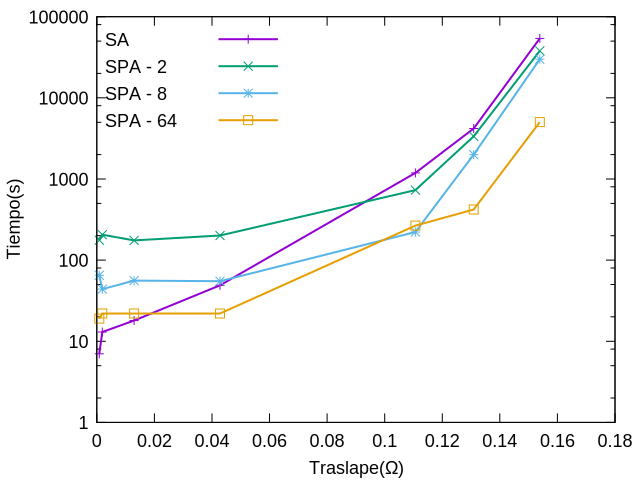
\includegraphics[width=4in]{graphs/traslape_mrg}
\caption{Tiempos de ejecución de $SA$ y $SPA$ utilizando 2, 8 y 64 hilos bajo diferentes valores de $\Omega$ (escala logarítmica)}
\label{fig:traslape-a}
\end{figure}

\begin{figure}[hbtp]
\centering
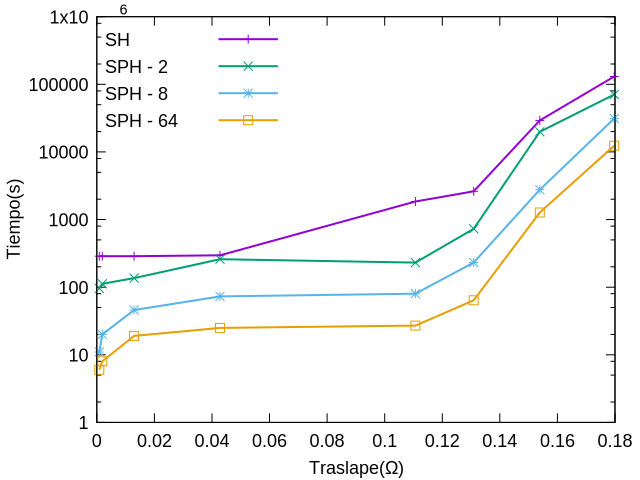
\includegraphics[width=4in]{graphs/traslape_hrg}
\caption{Tiempos de ejecución de $SH$ y $SPH$ utilizando 2, 8 y 64 hilos bajo diferentes valores de $\Omega$ (escala logarítmica)}
\label{fig:traslape-h}
\end{figure}

Es evidente que el valor del traslape $\Omega$ alcanzado en las redes que consideran el cumplimiento del $PC$ y las $RG$, es relativamente bajo ($\Omega<1$). Este hecho se debe a la restricción impuesta por las restricciones geométricas. Esto último se ilustra en las ecuaciones \ref{eq:eq02} y \ref{eq:eq03}:

\begin{equation}
B_C(R_S) \geq S(R_S)
\label{eq:eq02}
\end{equation}

\begin{eqnarray}
\nonumber \\
B_C(R_S) = & \{\int\limits^{R_S} ... \int\limits_{0} F_B(R_{B1})\; ... \; F_B(R_{BC})dR_{B1} \nonumber \\
& \; \ldots \; dR_{BC} \}^{1/C}
\label{eq:eq03}
\end{eqnarray}

donde $B_C(R_S)$ corresponde al volumen definido por la ecuación \ref{eq:eq03}; esta se relaciona con el conjunto de enlaces que pueden ser conectados a un sitio, evitando al mismo tiempo la existencia de interferencias entre ellos. $S(R_S)$ es la fracción de sitios que son de tamaño $R_S$ o más pequeños.\\

Las ecuaciones \ref{eq:eq02} y \ref{eq:eq03} restringen el valor de traslape como se muestra en \cite{ref5}, ya que la definición matemática de $B_C(R_S)$ impide en si alcanzar valores cercanos a la unidad, es por eso que los valores mostrados del traslape $\Omega<1$.\\

En la Figura \ref{fig:threads}, se muestran cuatro casos de comparación entre las soluciones $SPA$ y $SPH$ en términos del tiempo de construcción de una red porosa de tamaño $L=100$ con distintos traslapes y variando el número de hilos utilizados para la construcción de la red. En cada caso se añade como referencia dos líneas rectas que representan los tiempos de construcción de la red porosa con el traslape especificado para las soluciones $SA$ y $SH$.\\

En la Figura \ref{fig:threads60}, se muestra el primer caso para construcción de una red de tamaño $L=100$ con un  traslape de $\Omega=0.001908$, la solución $SPH$ muestra en general un mejor rendimiento que $SPA$ sin embargo muestra un bajo rendimiento respecto a $SA$ esto se debe a que al utilizar un traslape tan pequeño el número de violaciones a las $RG$ es bajo por lo cual la solución $SPH$ consume la mayor parte de su tiempo en la inicialización de la red particularmente en proceso de ordenamiento de sitios y enlaces mientras que $SA$ trabaja directamente en la eliminación de las violaciones, lo mismo ocurre con $SH$.\\

En la Figura \ref{fig:threads50}, se muestra el segundo caso para construcción de una red de tamaño $L=100$ con un  traslape de $\Omega=0.042809$, podemos ver que $SPA$ y $SPH$ muestran un compartimento muy similar en el cual a partir del uso de más de 8 hilos mejoran su rendimiento respecto a $SA$, al aumentar el traslape también aumenta el número de violaciones a las $RG$ lo que se transforma en mayor trabajo para cada hilo. Para $SPA$ en el caso anterior y en el actual(hasta 8 hilos) la mayor parte de tiempo se consumía en la distribución y redistribución de los datos es por eso que se muestra un rendimiento menor que $SA$. Para $SPH$ por las mismas causas tiene que un compartimento similar al del caso  sin embargo en este caso se obtuvo un redimiento mejor que el de $SA$ utilizando 8 hilos a diferencia de los 32 necesarios en el caso anterior.\\

En la Figura \ref{fig:threads43}, se muestra el tercer caso para construcción de una red de tamaño $L=100$ con un traslape de $\Omega=0.153895$, la solución $SPH$ muestra un mejor rendimiento que $SA$ y $SPA$ esto como consecuencia de dos factores el primero es que el traslape ocasiono un aumento significativo de violaciones a las $RG$ y el segundo es el proceso de inicialización que en $SA$ y $SPA$ es completamente aleatorio lo que hace que el número de violaciones a las $RG$ respecto a $SH$ y $SPH$ sea mucho mayor.\\

En la Figura \ref{fig:threads42}, se muestra el cuarto caso para construcción de una red de tamaño $L=100$ con un traslape de $\Omega=0.179723$, para este valor de traslape los tiempos de ejecución de las soluciones $SA$ y $SPA$ se incrementaron de forma exponencial por lo cual se interrumpió su ejecución. Para $SPH$ se pudo observar que en todos los casos siempre se mantuvo con un mejor rendimiento respecto a $SH$.\\

%\vfill
%\pagebreak
%%65	0.000862
%%60	0.001908 *
%%55	0.012969
%%50	0.042809 *
%%45	0.110658 *d
%%44	0.130928
%%43	0.153895
%%42	0.179723
\begingroup
\setlength{\parindent}{0cm}
\begin{figure}[hbtp]
\centering
\begin{tabular}{cc}
\subfloat[$\Omega=0.001908$]{
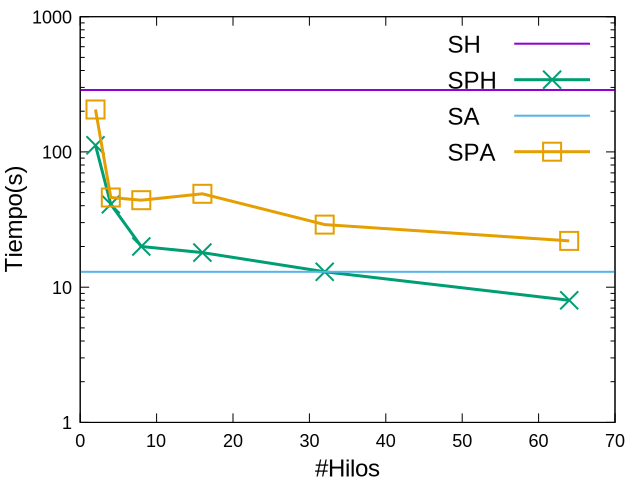
\includegraphics[width=2.7in]{graphs/threads60}
\label{fig:threads60}}
& \subfloat[$\Omega=0.042809$]{
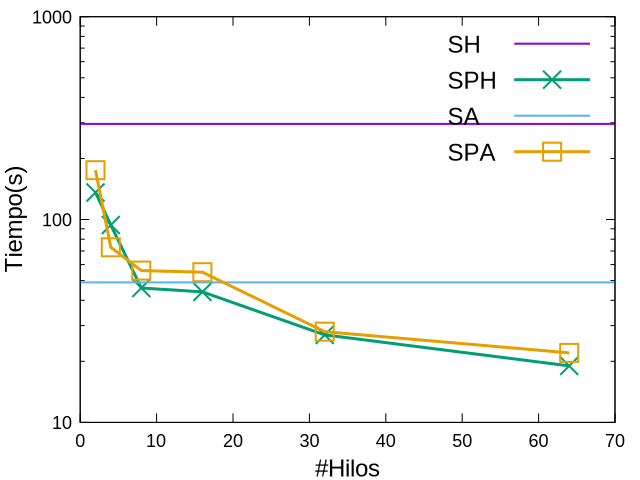
\includegraphics[width=2.7in]{graphs/threads50}
\label{fig:threads50}}\\
\subfloat[$\Omega=0.153895$]{
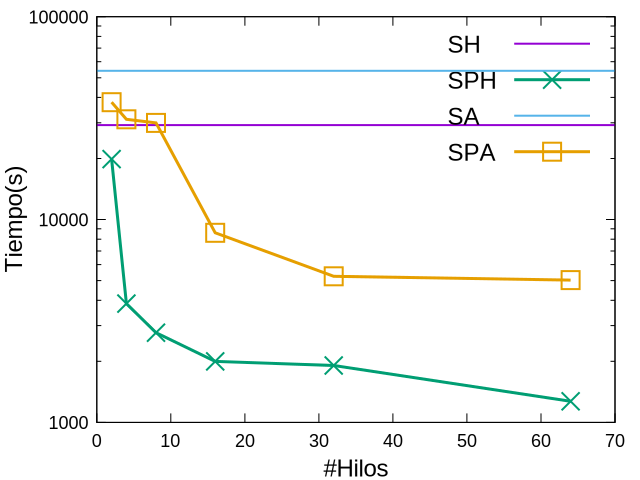
\includegraphics[width=2.7in]{graphs/threads43}
\label{fig:threads43}}
& \subfloat[$\Omega=0.179723$]{
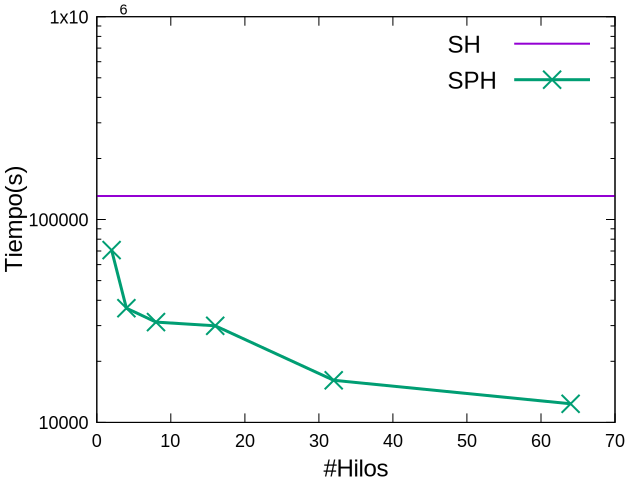
\includegraphics[width=2.7in]{graphs/threads42}
\label{fig:threads42}}
\end{tabular}
\caption{Tiempos de ejecución para $SH$, $SPH$, $SA$ y $SPA$ con distintos traslapes y variando el número de hilos(escala logarítmica)}
\label{fig:threads}
\end{figure}
\endgroup

\pagebreak
Cabe destacar que en todos los casos mostrados en la Figura \ref{fig:threads}, se utilizaron hasta 64 hilos en las pruebas lo cual supera al número cores o hilos de ejecución(hyperthreading) disponibles en el equipo de cómputo donde se realizaron las pruebas, sin embargo esta sobrecarga no efecto de forma negativa el rendimiento de las soluciones $SPA$ y $SPH$ si no al contrario, esto se debe a dos factores el primero es la naturaleza de los algoritmos utilizados en los cuales al particionar y operar sobre los datos no es necesaria una operación de reducción o unión esto da como resultado que la suma del tiempo de trabajar con conjuntos de datos más pequeños sea menor al tiempo que se necesitaría completar la misma tarea con un conjunto del tamaño de la suma de los conjuntos más pequeños, el segundo factor es la planificación de los hilos por parte del sistema operativo el cual puede manejar un numero de hilos superior al número cores o hilos de ejecución(hyperthreading). La mejora en tiempo con sobrecarga se obtuvo de forma constante utilizando hasta 64 hilos, al utilizar una valor más elevado se comenzaron a tener resultados impredecibles.\\

En la Figura \ref{fig:bignet} se muestran los tiempos de ejecución de la $SPH$ con $8$ hilos para la construcción de redes porosas de distintos tamaños con $L$ desde $100$ hasta $350$ y variando el traslape $\Omega$. En todos los casos de puede observar que conforme el traslape aumenta el tiempo de ejecución aumenta de forma muy similar para cualquier tamaño. Analizando estos resultados se pudo ver que el aumento en el tamaño de las redes no afecto de forma negativa al tiempo de ejecución final, el tiempo promedio para la sincronización y balanceo descrito en la sección \ref{sec:hybrid} para la $SPH$ fue menor a un segundo para redes con $L$ menor o igual a $200$ y para redes con $L$ mayor que $200$ y menor o igual a $350$ fue menor a dos segundos.

\begingroup
\setlength{\parindent}{0cm}
\begin{figure}[hbtp]
\centering
\begin{tabular}{cc}
\subfloat[$L=100$, $L=150$ y $L=200$]{
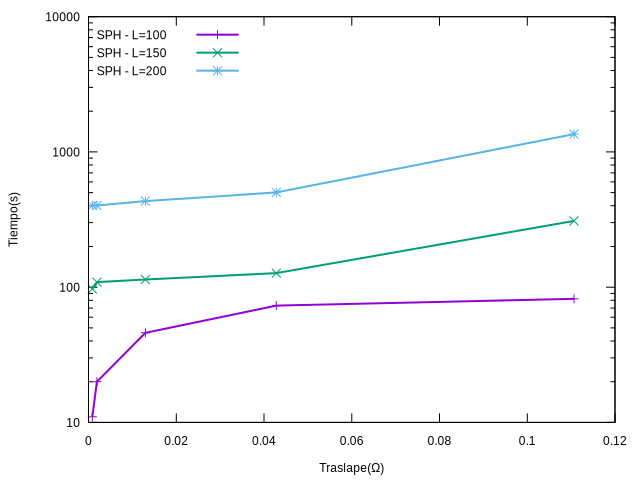
\includegraphics[width=2.7in]{graphs/bignet01}
\label{fig:bignet01}}
& \subfloat[$L=250$, $L=300$ y $L=350$]{
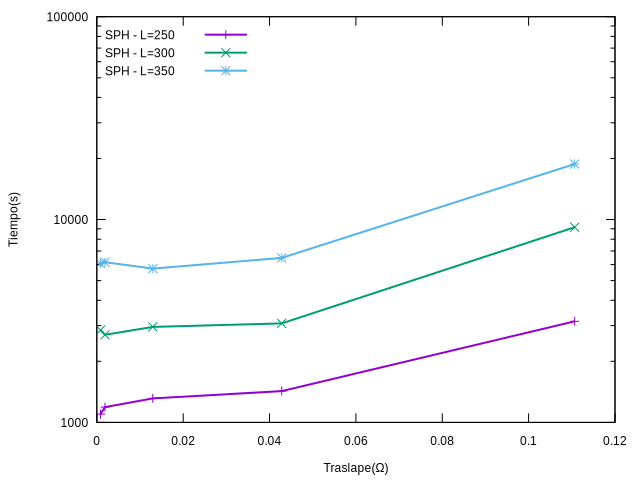
\includegraphics[width=2.7in]{graphs/bignet02}
\label{fig:bignet02}}\\
\end{tabular}
\caption{Tiempos de ejecución para $SPH$ para redes de distinto tamaño y variando el traslape (escala logarítmica)}
\label{fig:bignet}
\end{figure}
\endgroup


En las Figuras \ref{fig:networksomega}, \ref{fig:networksthreads} y \ref{fig:bignetworks} se muestran algunos ejemplos de redes porosas creadas utilizando  $SPH$, en estas imágenes se utilizó el siguiente código de colores: los poros grandes se muestran de color rojo, los poros de tamaño medio de color azul y los poros pequeños en color azul claro(cian). El código de colores nos permite visualizar como están distribuidos los poros a lo largo de la red.\\

En la Figura \ref{fig:networksomega} se muestran tres ejemplos de redes porosas de tamaño $L=100$ antes y después de eliminar las violaciones a las $RG$ utilizando diferentes traslapes y 8 hilos, se puede observar que en las Figuras \ref{fig:network60o} y \ref{fig:network50o} que una vez que se eliminaron las violaciones a las $RG$ en ambos casos se obtuvo una red porosa con una buena isotropía sin embargo en el caso de la Figura \ref{fig:network45o} en donde el traslape fue mayor y se puede apreciar como los poros grandes y medianos tienden a agruparse esto se debe a que a mayor traslape se tiene un número mayor de violaciones a las $RG$ y por consiguiente los intercambios de los pasos $MMC$-Paralelos descritos en la Sección \ref{subsec:pvalid}  sean más complicados.\\


\begingroup
\setlength{\parindent}{0cm}
\begin{figure}[hbtp]
\centering
\begin{tabular}{ccc}
\includegraphics[width=1.8in,height=1.8in]{networks/Gplot3D_L100_xmb26_xms60_s6_cs30_nc32_nt8_s_0bat}
& 
\includegraphics[width=1.8in,height=1.8in]{networks/Gplot3D_L100_xmb26_xms50_s6_cs30_nc32_nt8_s_0bat}
&
\includegraphics[width=1.8in,height=1.8in]{networks/Gplot3D_L100_xmb26_xms45_s6_cs30_nc32_nt8_s_0bat}
\\
\subfloat[$\Omega=0.001908$]{
\includegraphics[width=1.8in,height=1.8in]{networks/Gplot3D_L100_xmb26_xms60_s6_cs30_nc32_nt8_c_120bat}
\label{fig:network60o}}
& \subfloat[$\Omega=0.042809$]{
\includegraphics[width=1.8in,height=1.8in]{networks/Gplot3D_L100_xmb26_xms50_s6_cs30_nc32_nt8_c_140bat}
\label{fig:network50o}}
& \subfloat[$\Omega=0.110658$]{
\includegraphics[width=1.8in,height=1.8in]{networks/Gplot3D_L100_xmb26_xms45_s6_cs30_nc32_nt8_c_140bat}
\label{fig:network45o}}
\end{tabular}
\caption{Redes porosas antes y después de eliminar las violaciones a las $RG$ con diferentes valores de $\Omega$}
\label{fig:networksomega}
\end{figure}
\endgroup

En la Figura \ref{fig:networksthreads} se muestran las redes porosas generadas con tamaño  $L=100$  y con un traslape $\Omega=0.110658$  antes y después de eliminar las violaciones a las $RG$ utilizando $2$, $8$ y $64$ hilos respectivamente. Se puede apreciar que conforme se utiliza un mayor número de hilos la isotropía de las redes mejora esto se debe al cambio de origen en las etapas de sembrado de sitios y en los pasos $MMC$-Paralelos ambos descritos en las secciones \ref{subsec:pseeding} y  \ref{subsec:pvalid} respectivamente. A partir de lo anterior podemos ver que la solución $SPH$ además de mejorar el tiempo de ejecución se mejora la isotropía de las redes creadas conforme se utiliza un número mayor de hilos.\\

Por ultimo en la Figura \ref{fig:bignetworks} se muestran las redes generadas antes y después de eliminar las violaciones a las $RG$ con un tamaño $L$ de $150$, $250$ y $350$ respectivamente, en todos los casos se utilizó un el traslape $\Omega=0.110658$  y se utilizaron 8 hilos para la creación.\\

\begingroup
\setlength{\parindent}{0cm}
\begin{figure}[hbtp]
\centering
\begin{tabular}{ccc}
\includegraphics[width=1.8in,height=1.8in]{networks/Gplot3D_L100_xmb26_xms45_s6_cs30_nc32_nt2_s_0bat}
& 
\includegraphics[width=1.8in,height=1.8in]{networks/Gplot3D_L100_xmb26_xms45_s6_cs30_nc32_nt8_s_0bat}
&
\includegraphics[width=1.8in,height=1.8in]{networks/Gplot3D_L100_xmb26_xms45_s6_cs20_nc96_nt64_s_0bat}
\\
\subfloat[$2$ hilos]{
\includegraphics[width=1.8in,height=1.8in]{networks/Gplot3D_L100_xmb26_xms45_s6_cs30_nc32_nt2_c_120bat}
\label{fig:network2t}}
& \subfloat[$8$ hilos]{
\includegraphics[width=1.8in,height=1.8in]{networks/Gplot3D_L100_xmb26_xms45_s6_cs30_nc32_nt8_c_140bat}
\label{fig:network8t}}
& \subfloat[$64$ hilos]{
\includegraphics[width=1.8in,height=1.8in]{networks/Gplot3D_L100_xmb26_xms45_s6_cs20_nc96_nt64_c_180bat}
\label{fig:network64t}}
\end{tabular}
\caption{Redes porosas antes y después de eliminar las violaciones a las $RG$ utilizando un número diferente de hilos}
\label{fig:networksthreads}
\end{figure}
\endgroup

\begingroup
\setlength{\parindent}{0cm}
\begin{figure}[hbtp]
\centering
\begin{tabular}{ccc}
\includegraphics[width=1.8in,height=1.8in]{networks/Gplot3D_L150_xmb26_xms45_s6_cs30_nc100_nt8_s_0bat}
& 
\includegraphics[width=1.8in,height=1.8in]{networks/Gplot3D_L250_xmb26_xms45_s6_cs30_nc462_nt8_s_0bat}
&
\includegraphics[width=1.8in,height=1.8in]{networks/Gplot3D_L350_xmb26_xms45_s6_cs30_nc1270_nt8_s_0bat}
\\
\subfloat[$L=150$]{
\includegraphics[width=1.8in,height=1.8in]{networks/Gplot3D_L150_xmb26_xms45_s6_cs30_nc100_nt8_c_0bat}
\label{fig:bignetwork150}}
& \subfloat[$L=250$]{
\includegraphics[width=1.8in,height=1.8in]{networks/Gplot3D_L250_xmb26_xms45_s6_cs30_nc462_nt8_c_0bat}
\label{fig:bignetwork250}}
& \subfloat[$L=350$]{
\includegraphics[width=1.8in,height=1.8in]{networks/Gplot3D_L350_xmb26_xms45_s6_cs30_nc1270_nt8_c_0bat}
\label{fig:bignetwork350}}
\end{tabular}
\caption{Redes porosas antes y después de eliminar las violaciones a las $RG$ de diferentes tamaños}
\label{fig:bignetworks}
\end{figure}
\endgroup



%\pagebreak
%\begin{figure}[hbtp]
%\centering
%\includegraphics[width=4in]{img/variatraslape.pdf}
%\caption{Tiempos de ejecución de NoMISS, BSGR y BSGR paralelo, bajo diferentes valores de $\Omega$ (escala logarítmica)}
%\label{fig:timevartraslape}
%\end{figure}
%
%La Figura \ref{fig:timenuevo} muestra el timepo de ejecución requerido para crear una red porosa con $L=100$, $\Omega=0.15$, $ClusterSize=32$, y $NClusters=30$ utilizando un número de hilos diferente. El tiempo de ejecución en paralelo en general disminuye mientras aumenta el número de hilos. Podemos observar en algunos casos, como cuando el número e hilos  es igual a 6 y 14, el tiempo de ejecución no disminuye; creemos que estos casos se deben a la siembra aleatoria de clusters lo cual genera un número mayor de violaciones a las $RG$ que en los otros casos, al tener un mayor número de violaciones el tiempo que lleva generar una red porosa válida es mayor.\\
% 
%\begin{figure}[hbtp]
%\centering
%\includegraphics[width=4in]{img/tiempoPar2To16.pdf}
%\caption{Tiempos de ejecución de BSGR Paralelo utilizando de 2 a 16 hilos (escala logarítmica)}
%\label{fig:timenuevo}
%\end{figure}
%
%En la Figura \ref{fig:redes} observamos un ejemplo gráfico de una red porosa con $L=100$ y $\Omega=0.15$, obteniendo a partir de la versión BSGR (Figura \ref{fig:red1}), así como de la versión BSGR Paralela (Figura \ref{fig:red2}) utilizando 8 hilos. Estas imágenes representas redes porosas después del sembrado de cluster de poros y los pasos de asignación de enlaces; es decir, que se permite la existencia de violaciones a las $RG$. El código de color asignado en las Figuras \ref{fig:redes}, \ref{fig:redes2} y \ref{fig:redes3} es como sigue: los poros grandes se muestran de color rojo, los poros de tamaño medio de color azul y los poros pequeños en color azul claro.\\
%
%La Figura \ref{fig:redes2} muestra las anteriores redes porosas después de eliminar por completo las violaciones a las $RG$ a través de la aplicación de $MCs$. En las Figuras \ref{fig:red3} y \ref{fig:red4}, se puede observar que aun quedan estructuras de poro cúbicas que en redes porosas reales no se presentan.\\
%
%Después de aplicar un número adicional de $MCs$ le ísotropia de la red se mejora, obteniendo redes porosas que representan redes porosas más reales, como se muestra en las Figuras \ref{fig:red5} y \ref{fig:red6}.\\
%
%\begin{figure}[hbtp]
%\centering
%\begin{tabular}{cc}
%\subfloat[$ $]{
%\includegraphics[width=2.3in]{img/redsec100.png}
%\label{fig:red1}}
%& \subfloat[$ $]{
%\includegraphics[width=2.3in]{img/redpar100.png}
%\label{fig:red2}}
%\end{tabular}
%\caption{Redes porosas que permiten violaciones a las $GR$, con $L=100$ y $\Omega=0.15$, obtenidas con (a) BSGR y (b) BSGR Paralelo utilizando 8 hilos}
%\label{fig:redes}
%\end{figure}
%
%\begin{figure}[hbtp]
%\centering
%\begin{tabular}{cc}
%\subfloat[$ $]{
%\includegraphics[width=2.3in]{img/red3.png}
%\label{fig:red3}}
%& \subfloat[$ $]{
%\includegraphics[width=2.3in]{img/red4.png}
%\label{fig:red4}}
%\end{tabular}
%\caption{Redes porosas libre de violaciones a las $GR$, con $L=100$ y $\Omega=0.15$, obtenidas con (a) BSGR  and (b) BSGR Paralelo utilizando 8 hilos}
%\label{fig:redes2}
%\end{figure}
%
%%\begin{figure}[h]
%%\centering
%%\begin{tabular}{cc}
%%\subfloat[$ $]{
%%\includegraphics[width=1.5in]{img/red5.png}
%%\label{fig:red5}}
%%& \subfloat[$ $]{
%%\includegraphics[width=1.5in]{img/red6.png}
%%\label{fig:red6}}
%%\end{tabular}
%%\caption{Pore networks with additional application of $MCs$, obtained from the Parallel BSGR with $L=200$ and $\Omega=0.15$, (a) using 2 threads and (b) using 8 threads}
%%\label{fig:redes3}
%%\end{figure}
%
%\begin{figure}[t]
%\centering
%\begin{tabular}{cc}
%\subfloat[$ $]{
%\includegraphics[width=2.3in]{img/red7.png}
%\label{fig:red5}}
%& \subfloat[$ $]{
%\includegraphics[width=2.3in]{img/red8.png}
%\label{fig:red6}}
%\end{tabular}
%\caption{Redes porosas después de aplicar 2,000 $MCs$ adicionales, con L Pore networks after the application of 2000 additional $MCs$, con $L=100$ y $\Omega=0.15$, obtenidas con (a) BSGR  and (b) BSGR Paralelo utilizando 8 hilos}
%\label{fig:redes3}
%\end{figure}


	\chapter{Conclusiones y Trabajo Futuro}
\label{champ:conclusions}
\bigskip
\barra
\bigskip

%\textbf{Nota: Este apartado esta siendo traducido del artículo que se presentara en el workshop PDSEC 2014 2014 en el Conrgeso IEEE IPDPS 2014, adicionalmente se complementara con resultados de pruebas en progreso}.\\
%
%In this work, a basic solution, BSGR, to simulate pore networks under the existence of Geometrical Restrictions was proposed. This approach is a contribution in the study of more realistic pore materials. In order to offer an efficient solution, we also proposed a parallel version of BSGR. The parallel algorithm was designed by using a set of threads which cooperate in the construction of the pore network. A dynamic data partitioning was performed among the executing threads. Our results indicated that the proposed parallel algorithm outperformed its sequential counterpart, for example in a configuration with $L= 100$, $\Omega=0.13$ and using $16$ threads the acceleration obtained was $20.6$ times faster. Future work includes the design and comparison of different versions of our parallel solution using different architectures like clusters, multi-core processors and GPU's. 
	%%\bibliographystyle{plain}
%\pagestyle{plain}
\begin{appendices}
\chapter{Artículo IPDPS 2014}
\label{champ:appendices}
\bigskip
\barra
\bigskip
%\addtocontents{toc}{\protect\setcounter{tocdepth}{0}}
%\appendixpage
%\noappendicestocpagenum
%\addappheadtotoc
\includepdf[pages=-,pagecommand={},width=1.3\textwidth]{agonzalez-ipdps}
\end{appendices}
	\bibliographystyle{plain}
\begin{thebibliography}{9}
 \bigskip
 \barra
 \bigskip

\bibitem{ref1}
S. Cordero, et al., ''Review: Site-Bond Network Modeling of Disordered Porous Media,`` vol. 21, pp. 101–116, 2004.

\bibitem{ref2}
S. Cordero, F. Rojas, J.L. Riccardo, ''Simulation of three-dimensional porous networks,`` Colloids and Surfaces A: Physicochemical and Engineering Aspects, vol. 187–188, pp. 425-438, 2001. 

\bibitem{ref3}
G. Román, F. Rojas, M. Aguilar, S. Cordero, M.A. Castro, ''In-silico simulation of porous media: Conception and development of a greedy algorithm,`` Microporous and Mesoporous Materials, vol. 137, pp. 18-31, 2011. 

\bibitem{ref4}
J. Matadamas, G. Román-Alonso, F. Rojas, M. Castro, A. Boukerche, M. Aguilar, S. Cordero, ''Parallel Simulation of Pore Networks Using Multicore CPUs”, IEEE Transactions on Computers, 2012. 

\bibitem{ref5}
''Refinements of the Twofold Description of Porous Media``, Mayagoitia V., Rojas F., Kornhauser I.,Zgrablich G., Faccio R.J., Gilot B., and Guiglion C., Langmuir, 12, 211-216, 1996. 

\bibitem{ref6}
B. Chapman, G. Jost, R. van der Pas, ''Using OpenMP: Portable Shared Memory Parallel Programming,`` The MIT Press, pp. 384, 2007. 

\bibitem{ref7}
C.H. Moreno, F. Rojas, G. Román, S. Cordero, M.A. Castro, M. Aguilar, ''A Parallel Simulator for Mercury (Hg) Porosimetry,`` M. Ropo et al. (Eds.): EuroPVM/MPI 2009. LNCS, Springer, vol. 5759, pp. 294–304, 2009.

\bibitem{ref8}
M. Sahimi, ''Flow phenomena in rocks: from continuum models to fractals, percolation, cellular automata, and simulated annealing,`` Rev. Mod. Phys. 1993, 65(4), 1393-1534. 

\bibitem{ref9}
U. Gil-Cruz, M. A. Balderas-Altamirano, S. Cordero-Sánchez, ''Textural study of simulated dimorphic porous substrates,`` Colloids Surf. A, 2010, 357(1-3), 8492UTF$\{$2013$\}$90. 

\bibitem{ref10}
M.D. Kalugin, and A.V. Teplukhin, ''Parallel Monte Carlo study on caffeine-DNA interaction in aqueous solution``, IPDPS, pp.1-8, 2009 IEEE International Symposium on Parallel $\&$ Distributed IP Processing, 2009. 

\bibitem{ref11}
V. Mayagoitia, F. Rojas, I. Kornhauser and H. Pérez-Aguilar. ''Modeling of Porous Media and Surface Structures: Their True Essence as Networks,`` Langmuir. vol. 13, pp. 1327-1331 1997.

\bibitem{ref12} T. Sterling. ''Beowulf Cluster Computing with Linux,`` MIT Press, Cambridge, 2001.

\bibitem{ref13}
David R. Butenhof, ''Programming With Posix Threads,`` Addison-Wesley, 1997.

\bibitem{ref14}
H. Chung, C. Chang, H. Hsiao and Y. Chao, ''The Load Rebalancing Problem in Distributed File Systems,`` Cluster Computing (CLUSTER), IEEE International Conference on, pp.117,125, 24-28 Sept. 2012.

\bibitem{ref15}
M. Newman and G. Barkema, ''Monte Carlo Methods in Statistical Physics,`` Oxford University Press, Chap. 2, pp. 31-44, 2007.

\bibitem{ref16}
A. Gonz\'alez-M\'endez, G. Rom\'an-Alonso, F. Rojas-Gonz\'alez, M.A. Castro-Garc\'ia, M. Aguilar-Cornejo, and S. Cordero-S\'anchez;
''Construction of Porous Networks subjected to Geometric Restrictions by using OpenMP''; IEEE 28th
International Parallel \& Distributed Processing Symposium Workshops, Phoenix, USA, pp. 1189-1197, 2014.

%\bibitem{ref17}
%Fernando Rojas-Gonz\'alez, Graciela Rom\'an-Alonso, Salom\'on Cordero-S\'anchez, Miguel Alfonso Castro-Garc\'ia, Manuel Aguilar-Cornejo and Jorge Matadamas Hern\'andez; Book Chapter 1: ''On The Conception and Assessment of Mesopore Networks: Development of Computer Algorithms''; Nova Science Publishers, Inc. pp.1-28, to appear, 2014.

\bibitem{ref17}
Fernando Rojas-Gonz\'alez, Graciela Rom\'an-Alonso, Salom\'on Cordero-S\'anchez, Miguel Alfonso Castro-Garc\'ia, Manuel Aguilar-Cornejo and Jorge Matadamas Hern\'andez; Book "Comprehensive Guide for Mesoporous Materials"; Chapter : ''On The Conception and Assessment of Mesopore Networks: Development of Computer Algorithms''; Nova Science Publishers, Inc. vol. 3, pp.1-28, to appear (2o trimestre de 2015), ISBN: 978-1-63463-318-5, 2015.

\bibitem{ref18}
S. Cordero, F. Rojas, and J.L. Riccardo; "Simulation of three-dimensional porous networks Colloids and Surfaces A: Physicochemical and Engineering Aspects", 187-188 (2001), pp.425- 438, 2001.


%\bibitem{mchybrid}
%G. Tang, K. Li, H. Chen and J. Du, ''A Hybrid Parallel TRidiagonal Solver on Multi-Core Architectures,`` 2014 IEEE 28th International Parallel $\&$ Distributed Processing Symposium Workshops, pp.604-613, 19-23 Mayo 2014.
%
%\bibitem{mcmulticore}
%M. Mezmaz, R. Leroy, N. Melab and D. Tuyttens, ''A Multi-Core Parallel Branch-and-Bound Algorithm Using Factorial Number System,`` 2014 IEEE 28th International Parallel $\&$ Distributed Processing Symposium, pp.1203-1212, 19-23 Mayo 2014.
%
%\bibitem{mcdynamically}
%S. Donfack, S. Tomov and J. Dongarra, ''Dynamically balanced synchronization-avoiding LU factorization with multicore and GPUs,`` 2014 IEEE 28th International Parallel $\&$ Distributed Processing Symposium Workshops, pp.958-965, 19-23 Mayo 2014.
%
%\bibitem{mcopenmpt}
%A. Qawasmeh, A. Malik and B. Chapman, ''OpenMP Task Scheduling Analysis via OpenMP Runtime API and Tool Visualization,`` 2014 IEEE 28th International Parallel $\&$ Distributed Processing Symposium Workshops, pp.1049-1058, 19-23 Mayo 2014.
%
%\bibitem{mcscheduling}
%L. Chen, X. Huo, G. Agrawal, ''Scheduling Methods for Accelerating Applications on Architectures with Heterogeneous Cores,`` 2014 IEEE 28th International Parallel $\&$ Distributed Processing Symposium Workshops, pp.48-57, 19-23 Mayo 2014.
%
%\bibitem{sibalancing}
%C. Xu, L. Zhang, X. Deng, J. Fang, G. Wang, W. Cao, Y. Che, Y. Wang and W. Liu, ''Balancing CPU-GPU Collaborative High-order CFD Simulations on the Tianhe-1A Supercomputer,`` 2014 IEEE 28th International Parallel $\&$ Distributed Processing Symposium, pp.725-734, 19-23 Mayo 2014.
%
%\bibitem{sicloud}
%A. Paya and Dan C. Marinescu, ''Cloud-based Simulation of a Smart Power Grid
%,`` 2014 IEEE 28th International Parallel $\&$ Distributed Processing Symposium Workshops, pp.875-884, 19-23 Mayo 2014.
%
%\bibitem{siconstructing}
%J. Zola, ''Constructing Similarity Graphs from Large-scale Biological Sequence Collections,`` 2014 IEEE 28th International Parallel $\&$ Distributed Processing Symposium Workshops, pp.500-507, 19-23 Mayo 2014.
%
%\bibitem{sikdtree}
%K. Kofler, D. Steinhauser, B. Cosenza, I. Grasso, S. Schindler and T. Fahringer , ''Kd-tree Based N-Body Simulations with Volume-Mass Heuristic on the GPU,`` 2014 IEEE 28th International Parallel $\&$ Distributed Processing Symposium Workshops, pp.1256-1265, 19-23 Mayo 2014.
%
%\bibitem{silscale}
%X. Liu and E. Chow, ''Large-Scale Hydrodynamic Brownian Simulations on Multicore and Manycore Architectures,`` 2014 IEEE 28th International Parallel $\&$ Distributed Processing Symposium, pp.563-572, 19-23 Mayo 2014.
%
%\bibitem{sinfusion}
%N. Fujita, H. Nuga, T. Boku and Y. Idomura, ''Nuclear Fusion Simulation Code Optimization and Performance Evaluation on GPU Cluster,`` 2014 IEEE 28th International Parallel $\&$ Distributed Processing Symposium Workshops, pp.1266-1274, 19-23 Mayo 2014.
%
%\bibitem{siovercomming}
%J. Yeom, A. Bhatele, K. Bisset, E. Bohm, A. Gupta, L. Kale, M. Marathe, D. Nikolopoulos, M. Schulz and L. Wesolowski, ''Overcoming the Scalability Challenges of Epidemic Simulations on Blue Waters,`` 2014 IEEE 28th International Parallel $\&$ Distributed Processing Symposium, pp.755-764, 19-23 Mayo 2014.
%
%\bibitem{siprocess}
%J. Li, A. Salighehdar, N. Ganesan ''Process Simulation of Complex Biochemical Pathways in Explicit 3D Space Enabled by Heterogeneous Computing Platform,`` 2014 IEEE 28th International Parallel $\&$ Distributed Processing Symposium Workshops, pp.528-535, 19-23 Mayo 2014.

\end{thebibliography}
\end{document}
